\documentclass{irdbeamer}

\usepackage[
    backend=biber,
    style=authoryear-comp,
    maxcitenames=2, % max 2 authors before switching to et al.
    maxbibnames=4,
    uniquelist=false, % stays et al. when almost the same authors
    uniquename=false, % dose not bother when first name not written the same way everywhere
    date=year, % month does not appear in bibliography
    natbib=true, % use natbib synthax
    url=false, % remove url
    eprint=false % remove eprint
]{biblatex}

\addbibresource{refs.bib}

% % Define the color for citations
% \definecolor{citecolor}{gray}{0.5} % 0.5 is the gray level, adjust as needed

% % Redefine citation commands to include the color
% \renewcommand{\cite}[1]{\textcolor{citecolor}{\citet{#1}}}
% \renewcommand{\citep}[1]{\textcolor{citecolor}{\citep{#1}}}
% \renewcommand{\citet}[1]{\textcolor{citecolor}{\citet{#1}}}

\let\oldcite=\cite                                                              
\renewcommand{\cite}[1]{\textcolor[rgb]{.5,.5,.7}{\oldcite{#1}}}
\let\oldcitep=\citep                                                              
\renewcommand{\citep}[1]{\textcolor[rgb]{.5,.5,.7}{\oldcitep{#1}}}


\usepackage{tikz}


% \usepackage{amsmath} % for aligned
\usepackage{listofitems} % for \readlist to create arrays
\usetikzlibrary{arrows.meta} % for arrow size
\usetikzlibrary{calc,intersections}
\usepackage[outline]{contour} % glow around text
\contourlength{1.4pt}

% COLORS
\usepackage{xcolor}
\colorlet{myred}{red!80!black}
\colorlet{myblue}{blue!80!black}
\colorlet{mygreen}{green!60!black}
\colorlet{myorange}{orange!70!red!60!black}
\colorlet{mydarkred}{red!30!black}
\colorlet{mydarkblue}{blue!40!black}
\colorlet{mydarkgreen}{green!30!black}

% STYLES
\tikzset{
  >=latex, % for default LaTeX arrow head
  node/.style={thick,circle,draw=myblue,minimum size=22,inner sep=0.5,outer sep=0.6},
  node in/.style={node,green!20!black,draw=mygreen!30!black,fill=mygreen!25},
  node hidden/.style={node,blue!20!black,draw=myblue!30!black,fill=myblue!20},
  node convol/.style={node,orange!20!black,draw=myorange!30!black,fill=myorange!20},
  node out/.style={node,red!20!black,draw=myred!30!black,fill=myred!20},
  connect/.style={thick,mydarkblue}, %,line cap=round
  connect arrow/.style={-{Latex[length=4,width=3.5]},thick,mydarkblue,shorten <=0.5,shorten >=1},
  node 1/.style={node in}, % node styles, numbered for easy mapping with \nstyle
  node 2/.style={node hidden},
  node 3/.style={node out}
}
\def\nstyle{int(\lay<\Nnodlen?min(2,\lay):3)} % map layer number onto 1, 2, or 3

% for plots
\usepackage{pgfplots}
\pgfplotsset{compat=1.18}

\title{Brief History of Recent Deep Learning}
\subtitle{Formation IA Écologie}
\author[Paul Tresson]{\textbf{Paul Tresson}, Maximilien Servajean, Benjamin Bourel}
\date{\today} % or whatever the date you are presenting in is
\institute[Institut de Recherche pour le Développement]{UMR AMAP}

%\copyrightnotice{Published by Institut de Recherche pour le Développement, with permission}

% %% to add a background image for the title slide, uncomment here
% \usebackgroundtemplate{
%   \tikz[overlay, remember picture] \node[at=(current page.center)] {
%     \includegraphics[width=\paperwidth,height=\paperheight]{example-image-a}
%   };
% }


\usepackage{tikz}
\usetikzlibrary{overlay-beamer-styles}

\newcommand{\timeline}[1]{
    \begin{tikzpicture}[yscale=0.4, font=\tiny]
        % Timeline arrows
        % \newcommand{\timelinestart}{1990}
        % \newcommand{\timelinestop}{2030}
        % \draw[line width=.5mm,-latex,red!80!black] (0,+0.5) -- (0,-{\timelinestop-\timelinestart} +.5); % Does not work
        \draw[line width=.5mm,-latex,red!80!black] (0,+0.5) -- (0,-20 +.5); % First timeline arrow
        \draw[line width=.5mm,-latex,blue!80!black] (+.3,+0.5) -- (+.3,-20 +.5); % Second timeline arrow

        %% Years on the right to graduate ?
        \foreach \year in {2010,2015,...,2025} {
                \draw[gray,line width=.3mm] (0.3,{-(\year-2010)}) -- (0.4,{-(\year-2010)}); % Ticks
                \node[gray,anchor=west,align=left, rotate=-45] at (+0.4,{-(\year-2010)}) {\year}; % Description labels
        }
        % models
        \foreach \index/\year/\yshift/\text in {
            1/2012/00/AlexNet,
            3/2015/00/ResNet,
            5e/2013/00/LSTM,
            6/2017/00/Transformers,
            7/2018/00/GPTs,
            8/2021/00/ViTs
        }
        {
            % Render only if \index is less than or equal to #1
            \ifnum\index>#1\relax
                % Skip this entry
            \else
                \draw[red!80!black,line width=.3mm] (0,{-(\year-2010)}) -- (-0.2,{-(\year-2010)}); % Ticks
                \node[red!80!black,anchor=east,align=right, rotate=-45,yshift=-\yshift] at (-0.2,{-(\year-2010)}) {\text}; % Description labels
            \fi
        }
        
        % Second set of labels
        \foreach \index/\year/\yshift/\text in {
            2/2015/50/ImageNet,
            4/2017/50/Pascal VOC
        }
        {
            % Render only if \index is less than or equal to #1
            \ifnum\index>#1\relax
                % Skip this entry
            \else
                \draw[blue!80!black,line width=.3mm] (+0.3,{-(\year-2010)}) -- (-0.2,{-(\year-2010)}); % Ticks
                \node[blue!80!black,anchor=east,align=right, rotate=-45] at (-0.2,{-(\year-2010)}) {\text}; % Description labels
            \fi
        }
        
    \end{tikzpicture}
}

\begin{document}
\addlogo{logos/IRD_banner.png}
\addlogo{logos/AMAP_banner.png}
%\addlogo{example-image-a}
\maketitle

\usebackgroundtemplate{}

\begin{frame}{Reminder}
    \begin{figure}
        \centering
        \vspace{-1cm}
        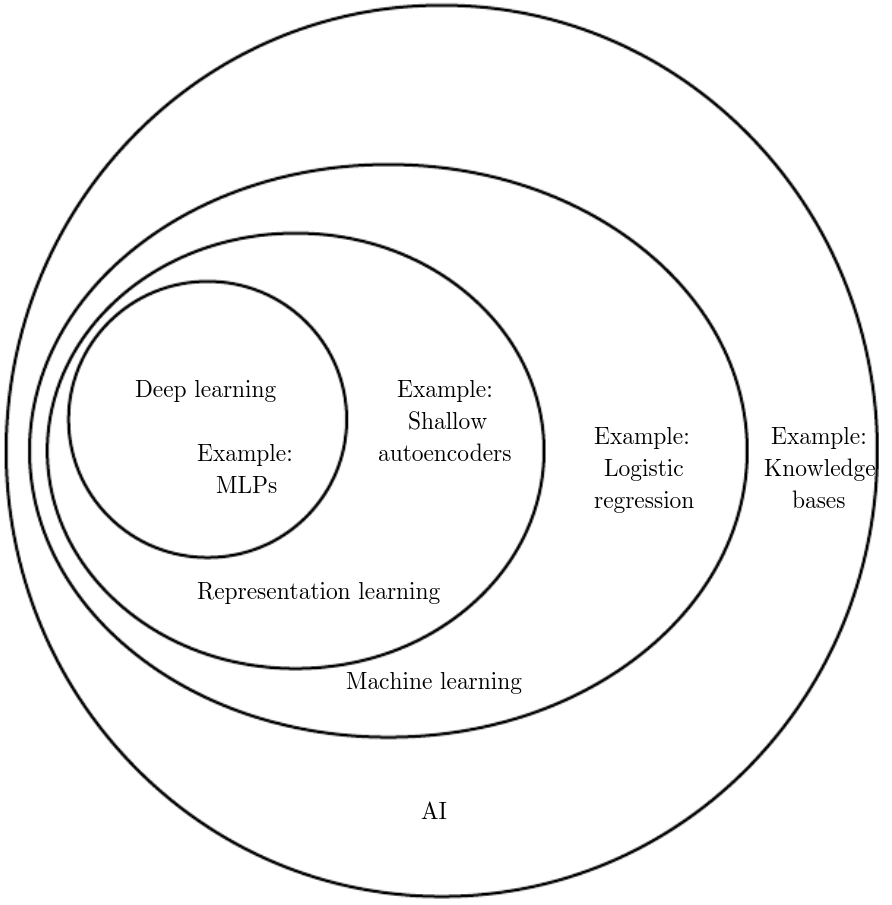
\includegraphics[width=0.45\linewidth]{figs/goodfellow_AI.png}
        \caption{\tiny Different types of Artificial Intelligence. From \cite{goodfellow2016deep}}
    \end{figure}
\end{frame}

% Années 1980 : Premiers Réseaux Neuronaux Profonds
% 1. Perceptron multicouche (MLP) - 1986
% Architecture : Perceptron multicouche avec une ou plusieurs couches cachées.
% Jeu de données paradigmatique : XOR Problem, un problème simple mais non linéaire qui ne peut pas être résolu par un perceptron simple. Ce problème a montré le besoin de couches cachées.
% Optimisation : Descente de gradient avec rétropropagation (algorithme introduit par Rumelhart, Hinton, et Williams en 1986). L'optimisation se fait en ajustant les poids grâce à la rétropropagation des erreurs à travers les couches.
\begin{frame}[t]{First Neural Network Model : The Perceptron}
    \begin{figure}
        \centering
        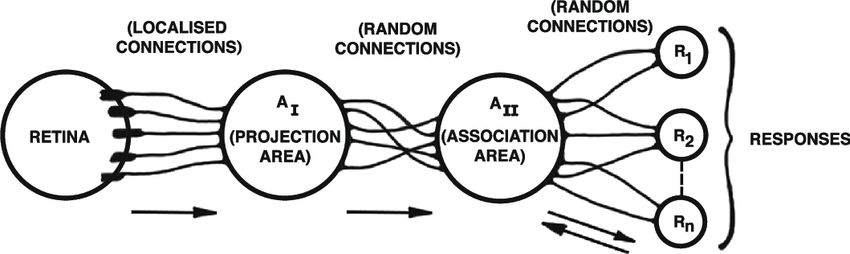
\includegraphics[width=\linewidth]{figs/perceptron.png}
        \caption{\tiny First probabilistic model of a neuron proposed by \cite{rosenblatt1958perceptron}}
    \end{figure}
\end{frame}

\begin{frame}[t]{First Neural Network Model : The Perceptron}
\centering
% \tikzset{int/.style = {draw, circle, fill=blue!20, minimum size=2em}}
% \begin{tikzpicture}[auto,>=latex]
%     % Input nodes
%     \node [int] (x1) {$x_1$};
%     \node [int, below of=x1, node distance=2cm] (x2) {$x_2$};
%     \node [below of=x2, node distance=1cm] (dots) {$\vdots$};
%     \node [int, below of=dots, node distance=1cm] (xn) {$x_n$};

%     % Hidden node
%     \node [int, right of=x2, node distance=4cm] (h1) {$\Sigma$};

%     % Output node
%     \node [int, right of=h1, node distance=4cm] (y) {$y$};

%     % Connections
%     \path[->] (x1) edge (h1)
%               (x2) edge (h1)
%               (xn) edge (h1);

%     \path[->] (h1) edge (y);
% \end{tikzpicture}

\tikzset{int/.style = {draw, circle, minimum size=2em}}
\begin{tikzpicture}[auto,>=latex]
    % Input nodes
    \node [int] (x1) {$x_1$};
    \node [int, below of=x1, node distance=2cm] (x2) {$x_2$};
    \node [below of=x2, node distance=1cm] (dots) {$\vdots$};
    \node [int, below of=dots, node distance=1cm] (xn) {$x_n$};

    % Hidden node
    \node [int, right of=x2, node distance=4cm] (h1) {$\Sigma$};

    % Output node
    \node [int, right of=h1, node distance=4cm] (y) {$y$};

    % Connections with labels
    \path[->] (x1) edge node {$w_1$} (h1)
              (x2) edge node {$w_2$} (h1)
              (xn) edge node {$w_n$} (h1);

    \path[->] (h1) edge (y);
\end{tikzpicture}
\end{frame}

\begin{frame}[t]{First Roadblock : XOR problem}
\begin{columns}
    \column{.4\linewidth}
    \begin{table}[]
    \large
        \centering
        \begin{tabular}{ccc}
             $x_{1}$&$x_{2}$&$y$  \\\hline
             0&0&\textcolor{blue}{0}\\
             1&0&\textcolor{red}{1}\\
             0&1&\textcolor{red}{1}\\
             1&1&\textcolor{blue}{0}\\
        \end{tabular}
    \end{table}
    \column{.6\linewidth}
    \begin{figure}
        \centering
        \includegraphics<1>[width=.8\linewidth]{figs/xor_margin.png}%
        \includegraphics<2>[width=.8\linewidth]{figs/xor_decision.png}
    \end{figure}
\end{columns}
\end{frame}


\begin{frame}[t]{1980's : First Deep Neural Networks}
\begin{columns}[t]
    \column{.4\linewidth}
    \vspace{1cm}
    \begin{itemize}
        \item<1-> Multi Layer Perceptron
        \item<2-> Non-linearity (\textit{e.g.} ReLu)
        \item<3-> Gradient Descent and Backpropagation\\ \cite{rumelhart1986learning}
    \end{itemize}
    \column{.6\linewidth}
    \only<1>{
    \begin{figure}
        \centering
        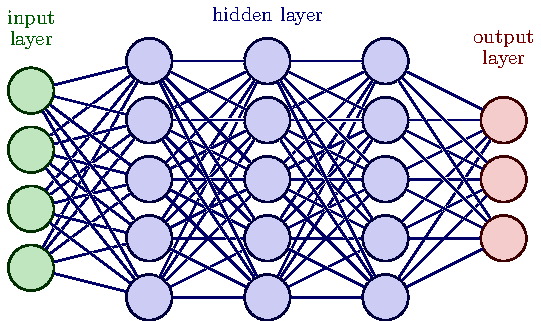
\includegraphics[width=\linewidth]{figs/mlp.pdf}
        \caption{\tiny Multi Layer Perceptron}
    \end{figure}
    }
    \only<2>{
    \begin{figure}
        \centering
        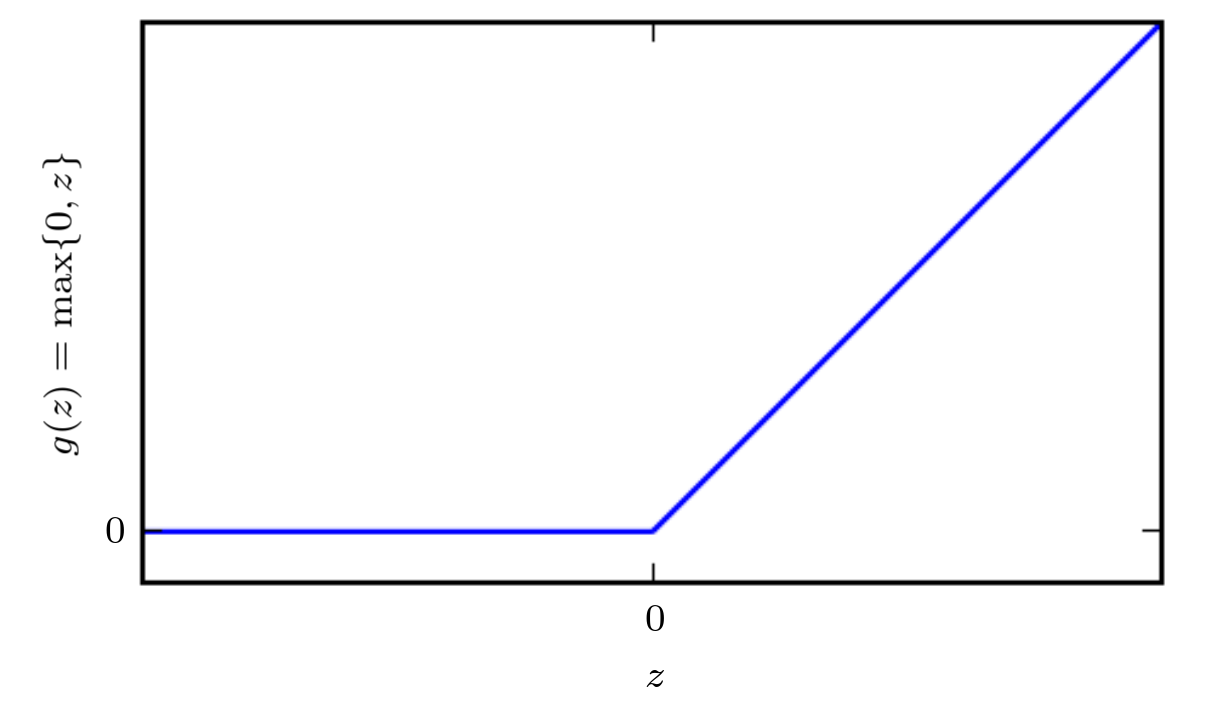
\includegraphics[width=\linewidth]{figs/relu.png}
        \caption{\tiny Rectified Linear Unit. Figure from \cite{goodfellow2016deep}}
    \end{figure}
    }
    \only<3->{
    \begin{figure}
        \centering
        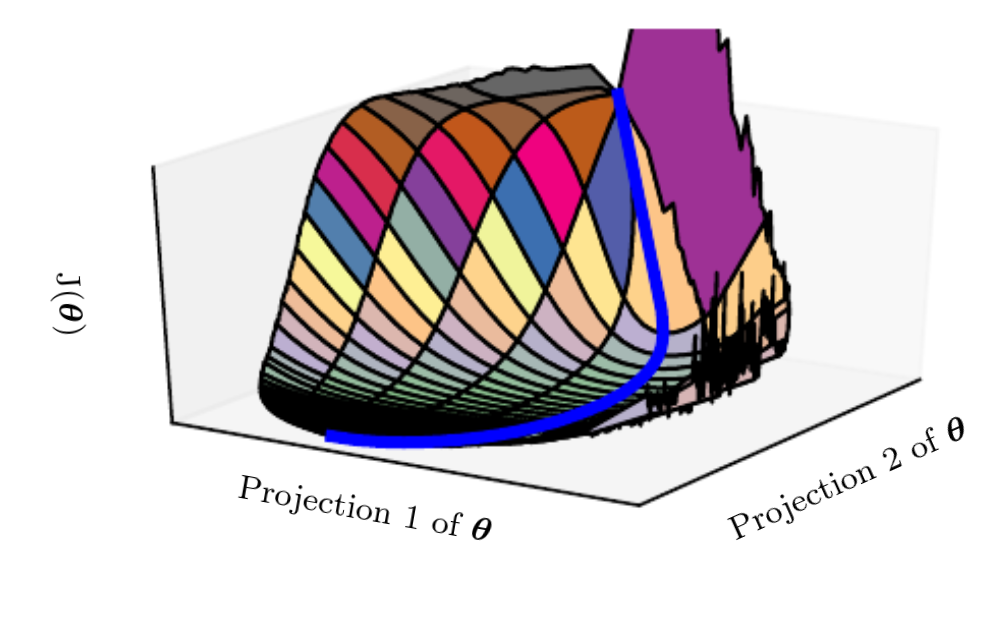
\includegraphics[width=\linewidth]{figs/SGD.png}
        \caption{\tiny Gradient descent example. Figure from \cite{goodfellow2016deep}}
    \end{figure}
    }
\end{columns}
\end{frame}



% Années 1990 : Avancées en Apprentissage Supervisé
% 2. Réseaux convolutifs (CNN) - 1998
% Architecture : LeNet-5 (Yann LeCun)
% Jeu de données paradigmatique : MNIST (digits handwritten)
% Optimisation : Descente de gradient stochastique (SGD) avec rétropropagation. SGD, qui calcule les gradients sur des mini-lots de données, a permis de rendre l'optimisation plus rapide et plus stable pour des réseaux convolutifs profonds.
% LeNet est devenu célèbre pour son application à la reconnaissance de chiffres manuscrits, ouvrant la voie aux architectures convolutives modernes.
\begin{frame}[t]{1990's : First Successes}
\begin{columns}[t]
    \column{.4\linewidth}
    \vspace{1cm}
    \begin{itemize}
        \item<1-> MNIST\\ \cite{lecun1998mnist}
        \item<2-> LeNet\\ \cite{lecun1989backpropagation}
        \item<3-> Convolutional Neural Network (CNN)\\ \cite{lecun1989generalization}
    \end{itemize}
    \column{.6\linewidth}
    \only<1>{
    \begin{figure}
        \centering
        \vspace{-1cm}
        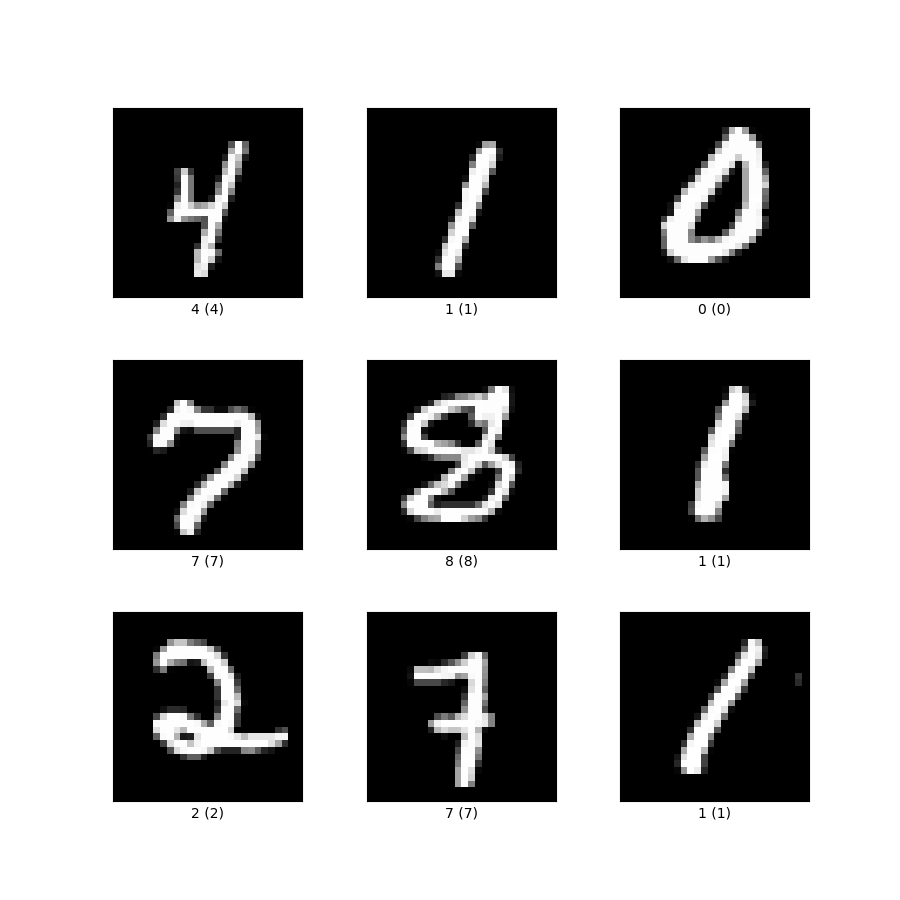
\includegraphics[width=.6\linewidth]{figs/mnist.png}
        \caption{\tiny Images from MNIST}
    \end{figure}
    }
    \only<2>{
    \begin{figure}
        \centering
        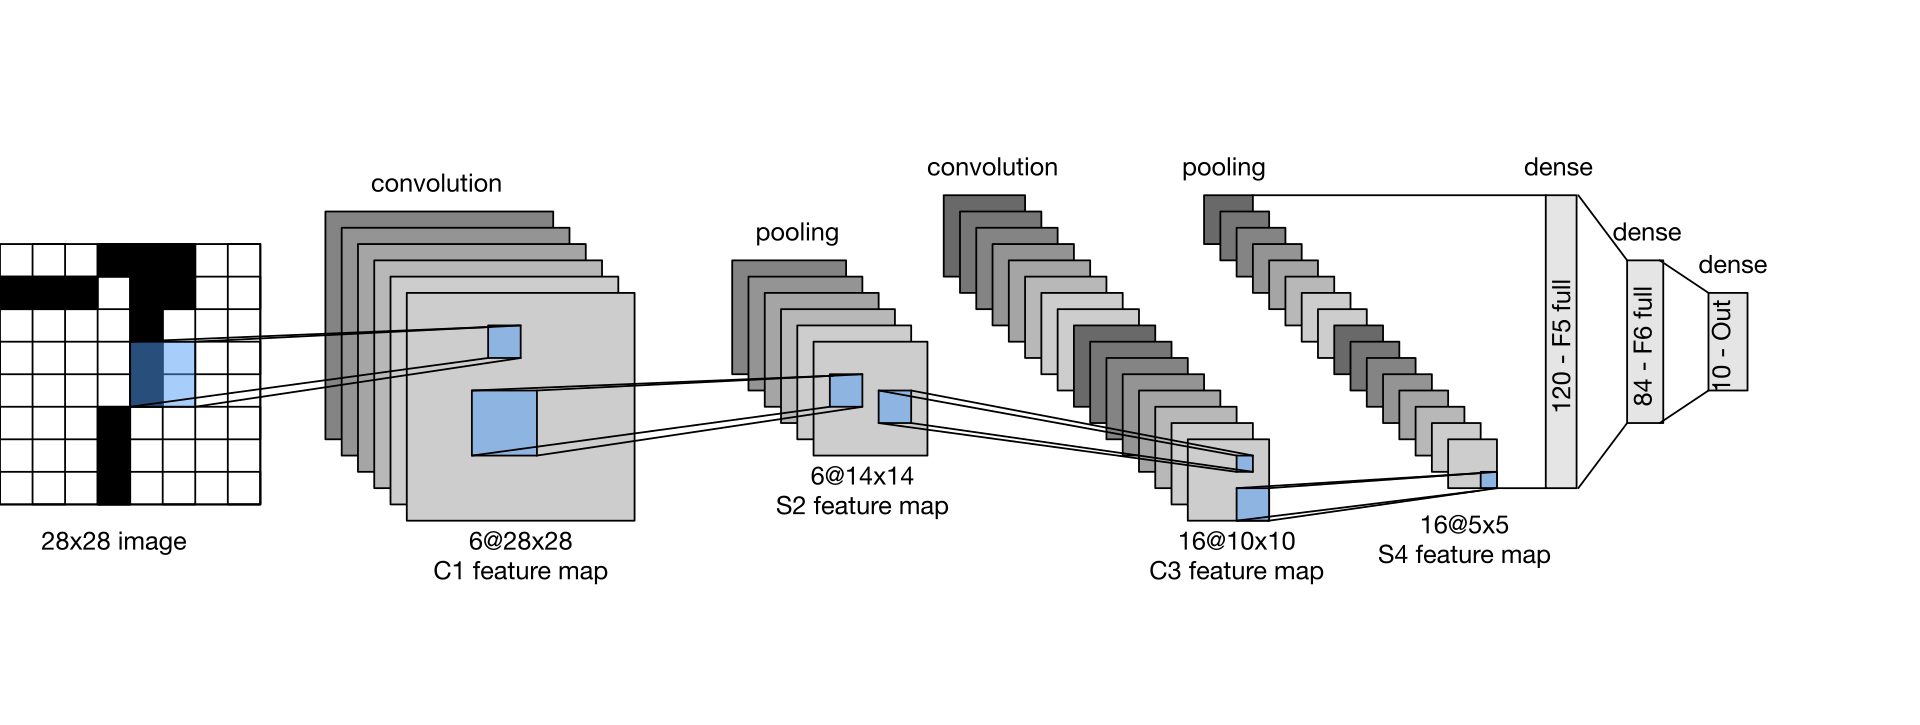
\includegraphics[width=\linewidth]{figs/LeNet.png}
        \caption{\tiny LeNet5.\\ Figure from Zhang et al. - \url{https://github.com/d2l-ai/d2l-en}}
    \end{figure}
    }
    \only<3->{
    \begin{figure}
        \centering
        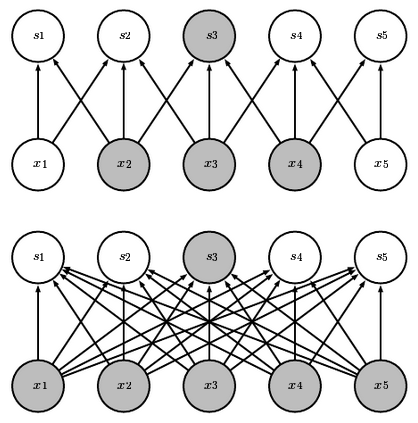
\includegraphics[width=.5\linewidth]{figs/cnn_sparse.png}
        \caption{\tiny sparse connectivity with CNNs.\\ Figure from \cite{goodfellow2016deep}}
    \end{figure}
    }
\end{columns}\nonumbernote{\tiny Modified National Institute of Standards and Technology} 
\end{frame}

\begin{frame}[t]{}
\textbf{\large Good proof of concept but too costly in computing power and datasets}
    \begin{figure}
        \centering
        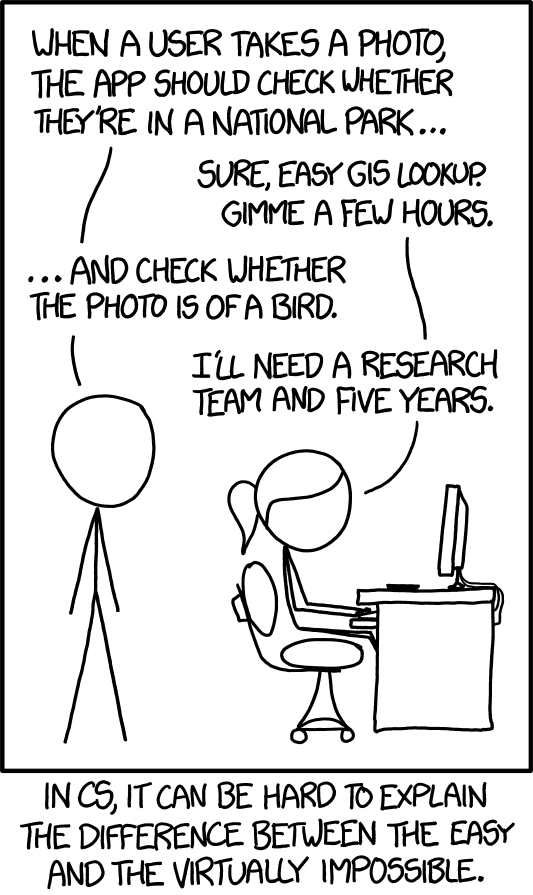
\includegraphics[width=.27\linewidth]{figs/xkcd_photo_is_a_bird.png}
    \vspace{-.5cm}
        \caption{\tiny XKCD comic from 2014}
    \end{figure}
\end{frame}
\begin{frame}[t]{}
\textbf{\large Good proof of concept but too costly in computing power and datasets}
\textbf{\large  ...until}

% \vspace{1cm}
% \hspace{.5cm}
% \begin{tabular}{llr}
%     \only<2->{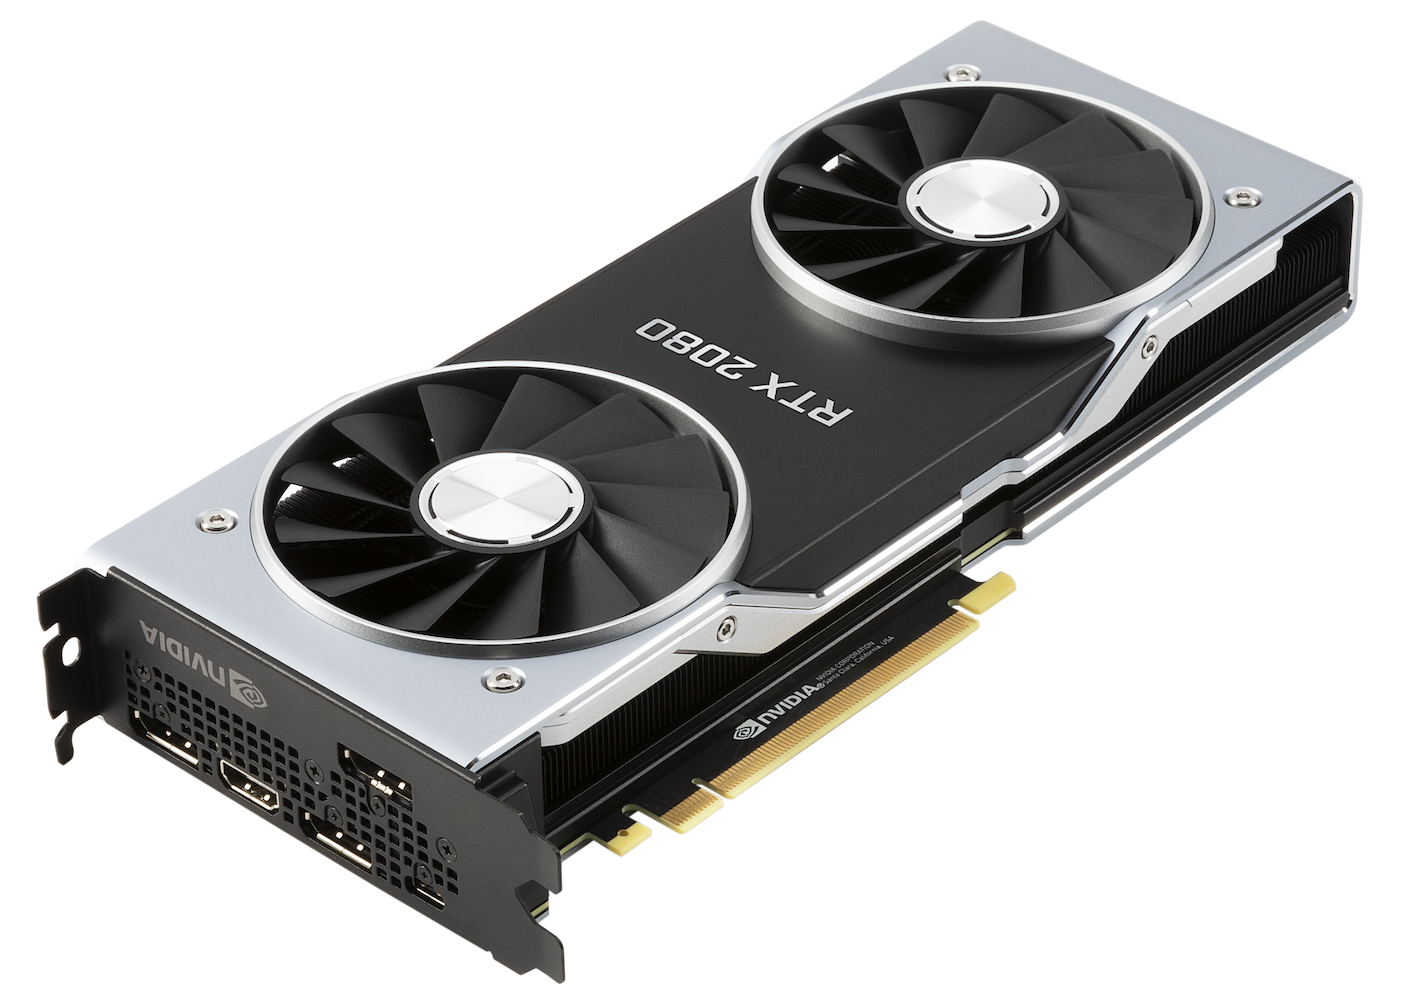
\includegraphics[width=.5\textwidth]{figs/gpu.png}}& &
%     \only<3->{\vspace{-.5cm}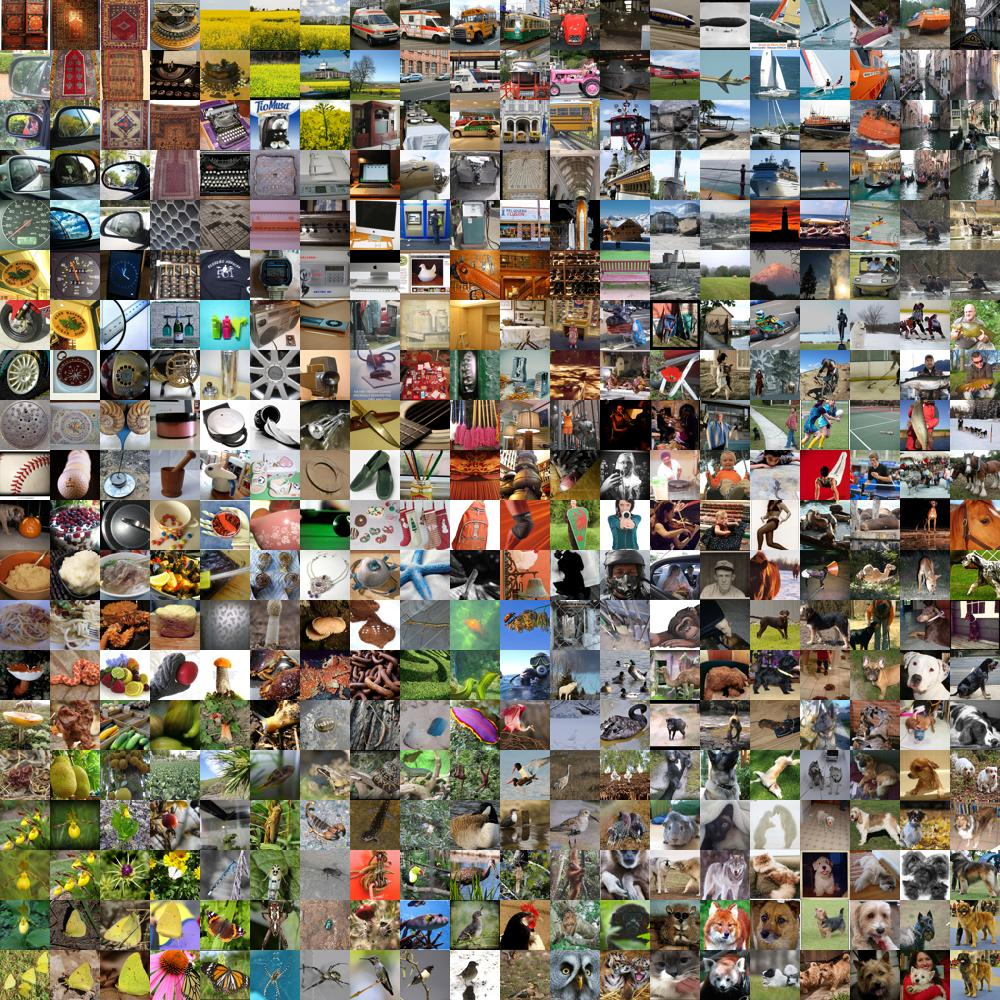
\includegraphics[width=.4\textwidth]{figs/imagenet-sample.jpg}}\\
% \end{tabular}
\end{frame}
\begin{frame}[t]{}
\textbf{\large Good proof of concept but too costly in computing power and datasets}
\textbf{\large  ...until}
\begin{center}
    \begin{tikzpicture}
        \node (img1) {{\visible<1->{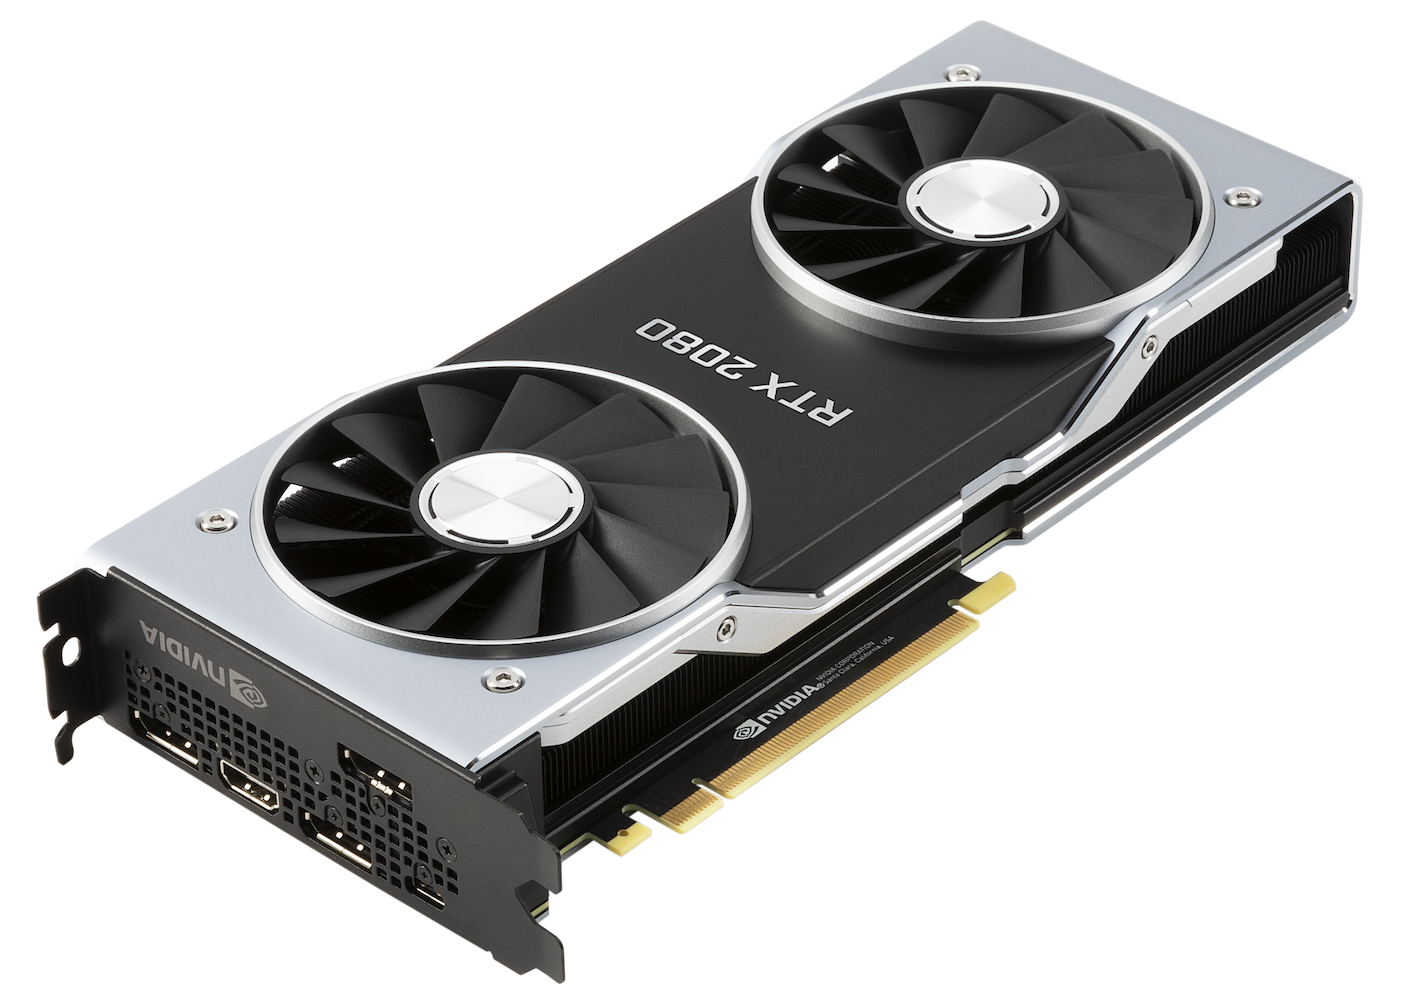
\includegraphics[width=.5\textwidth]{figs/gpu.png}}}};
        \node (img2) at (img1.south east) {{\visible<2>{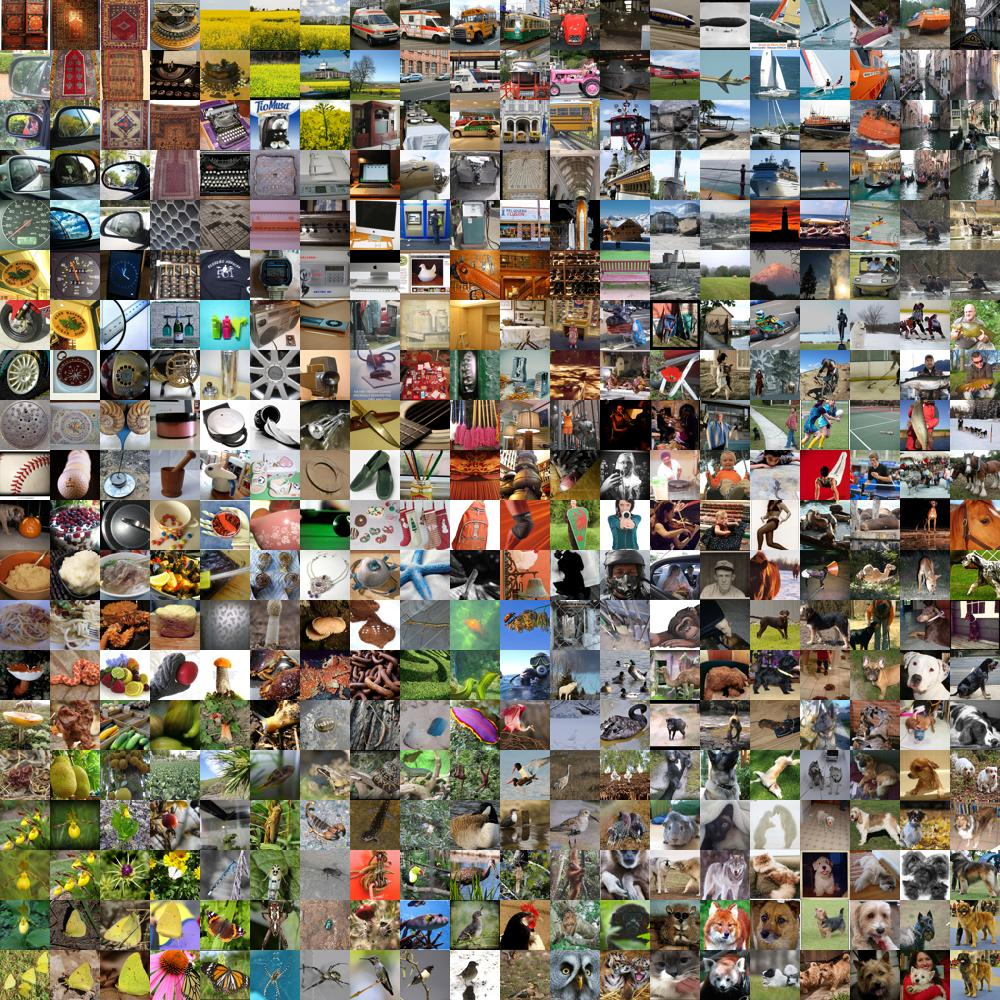
\includegraphics[width=.4\textwidth]{figs/imagenet-sample.jpg}}}};
    \end{tikzpicture}
\end{center}
\end{frame}




% Années 2000 : Renaissance et Apprentissage Profond
% 3. Réseaux de neurones à croyances profondes (DBN) - 2006
% Architecture : Deep Belief Network (DBN) (Hinton, Osindero, Teh)
% Jeu de données paradigmatique : MNIST
% Optimisation : Pré-entraînement non-supervisé via des Machines de Boltzmann restreintes (RBM), suivi d'une optimisation supervisée en utilisant la descente de gradient. Cette approche a relancé l'intérêt pour les réseaux profonds en permettant un pré-entraînement couche par couche qui stabilise l'apprentissage des réseaux très profonds.
% Les DBN ont montré comment les réseaux neuronaux pouvaient être pré-entraînés pour surmonter les problèmes de gradient vanishing dans les réseaux profonds.
% 4. Auto-encodeurs - 2006-2008
% Architecture : Auto-encodeurs profonds
% Jeu de données paradigmatique : CIFAR-10
% Optimisation : Utilisation d'auto-encodeurs pour pré-entraînement non-supervisé, puis raffinage supervisé avec SGD.

% Années 2010 : Explosion des Performances du Deep Learning
% 5. AlexNet (CNN Profond) - 2012
% Architecture : AlexNet (Krizhevsky, Sutskever, Hinton)
% Jeu de données paradigmatique : ImageNet (ILSVRC 2012)
% Optimisation : SGD avec momentum, et utilisation intensive de GPU pour accélérer le calcul. AlexNet a aussi introduit des techniques comme le Dropout pour réduire le sur-apprentissage, et l'activation ReLU (Rectified Linear Unit) pour éviter les problèmes de gradient vanishing.
% AlexNet est souvent crédité de la révolution du deep learning moderne grâce à sa performance sans précédent sur le benchmark ImageNet, réduisant l'erreur top-5 de 25,7% à 16,4%.
\begin{frame}[t]{2010's : CNN revolution}
\begin{columns}[t]
    \column{.4\linewidth}
    \begin{itemize}
        \item<1-> ImageNet\\ \cite{deng2009imagenet}
        \item<2-> AlexNet\\ \cite{krizhevsky2012imagenet}
        \item<3-> ResNet\\ \cite{he2016deep}
        \item<5-> YOLO, mask-RCNN...\\ \cite{redmon2016you,he2017mask}
    \end{itemize}
    \column{.6\linewidth}
    \only<1>{
    \begin{figure}
        \centering
        
\includegraphics[width=.7\linewidth]{figs/imagenet.png}
        \caption{}
    \end{figure}
    }
    \only<2>{
    \begin{figure}
        \centering
        \vspace{1cm}
        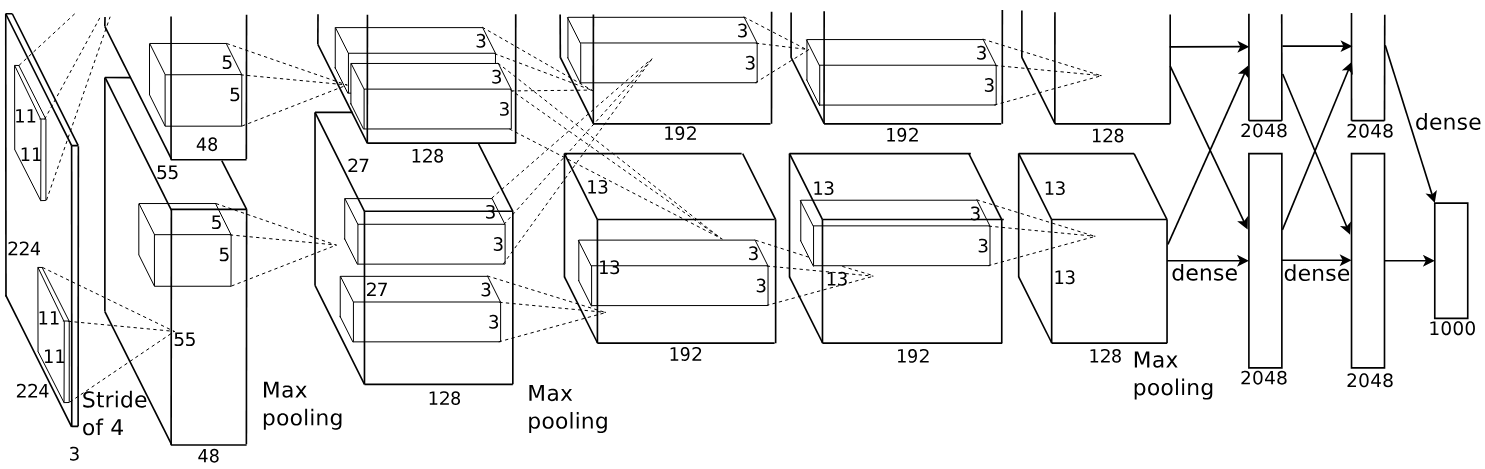
\includegraphics[width=.7\linewidth]{figs/alexnet}
        \caption{\tiny AlexNet. Figure from \cite{krizhevsky2012imagenet}}
    \end{figure}
    }
    \only<3-4>{
    \begin{figure}
        \centering
        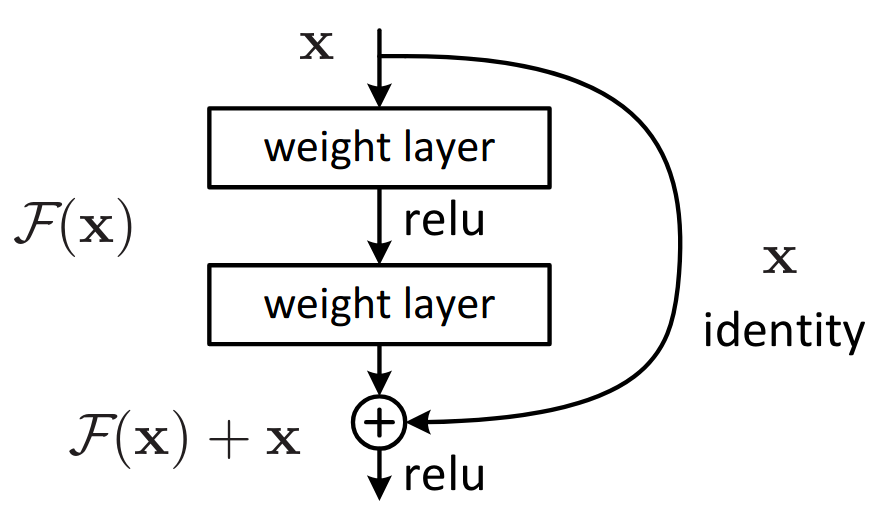
\includegraphics[width=.7\linewidth]{figs/resnet.png}
        \caption{\tiny A residual connection. Figure from \cite{he2016deep}}
    \end{figure}
    }
    \only<5>{
    \begin{figure}
        \centering
        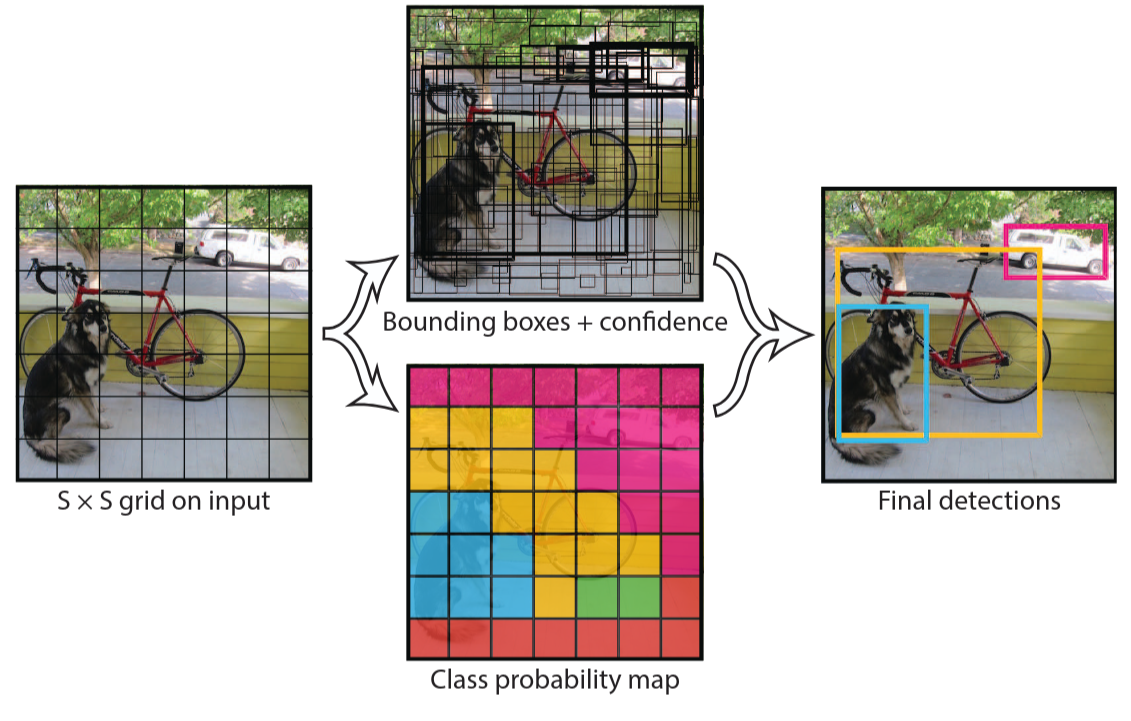
\includegraphics[width=.7\linewidth]{figs/yolo.png}
        \caption{\tiny YOLO. Figure from \cite{redmon2016you}}
    \end{figure}
    }
\end{columns}
    \only<4>{
        \centering
        \vspace{-0.5cm}
            \fbox{
\includegraphics[width=.7\paperwidth,]{figs/he_wiki.png}}
    }
\end{frame}


% 6. ResNet (Réseaux Résiduels) - 2015
% Architecture : ResNet (He et al.)
% Jeu de données paradigmatique : ImageNet (ILSVRC 2015)
% Optimisation : SGD avec momentum et initialisation spécifique des poids (He initialization). L'architecture résiduelle a introduit les skip connections (connexions de saut) pour atténuer les problèmes de gradient vanishing dans les réseaux très profonds (plus de 100 couches).
% ResNet a été un tournant dans l'augmentation de la profondeur des réseaux en introduisant des chemins de dérivation, ce qui a permis un apprentissage plus stable.
% 7. Réseaux récurrents (LSTM) - 2013-2015
% Architecture : LSTM (Long Short-Term Memory) (Hochreiter et Schmidhuber, popularisé par Sutskever, Graves, et autres)
% Jeu de données paradigmatique : Babi (questions answering), IMDB (sentiment analysis)
% Optimisation : SGD, parfois avec RMSProp ou Adam, et techniques de gestion des gradients comme le gradient clipping pour éviter les explosions de gradients dans les séquences longues.
% LSTM a dominé les tâches de séquence, telles que la traduction automatique, la génération de texte et l'analyse de sentiments.
\begin{frame}[t]{2010's : NLP}
\begin{columns}[t]
    \column{.4\linewidth}
    \vspace{1cm}
    \begin{itemize}
        \item<1-> IMBD\\ \cite{maas2011learning}
        \item<2-> LSTM\\ \cite{hochreiter1997long}
        \item<3-> RNN's\\ \textit{e.g.} \cite{sutskever2014sequence}
    \end{itemize}
    \column{.6\linewidth}
    \vspace{1cm}
    \only<1>{
    \begin{figure}
        \centering
        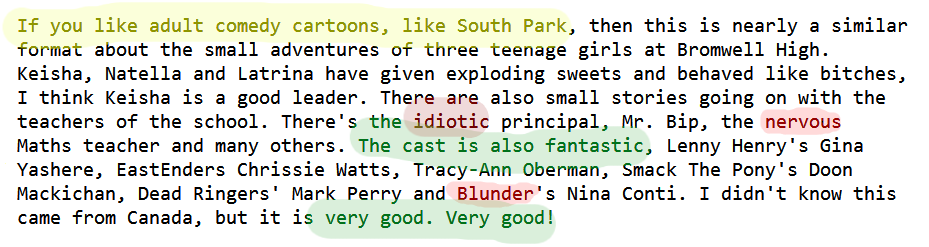
\includegraphics[width=\linewidth]{figs/IMDB.png}
        \caption{\tiny Extract from IMDB database}
    \end{figure}
    }
    \only<2>{
    \begin{figure}
        \centering
        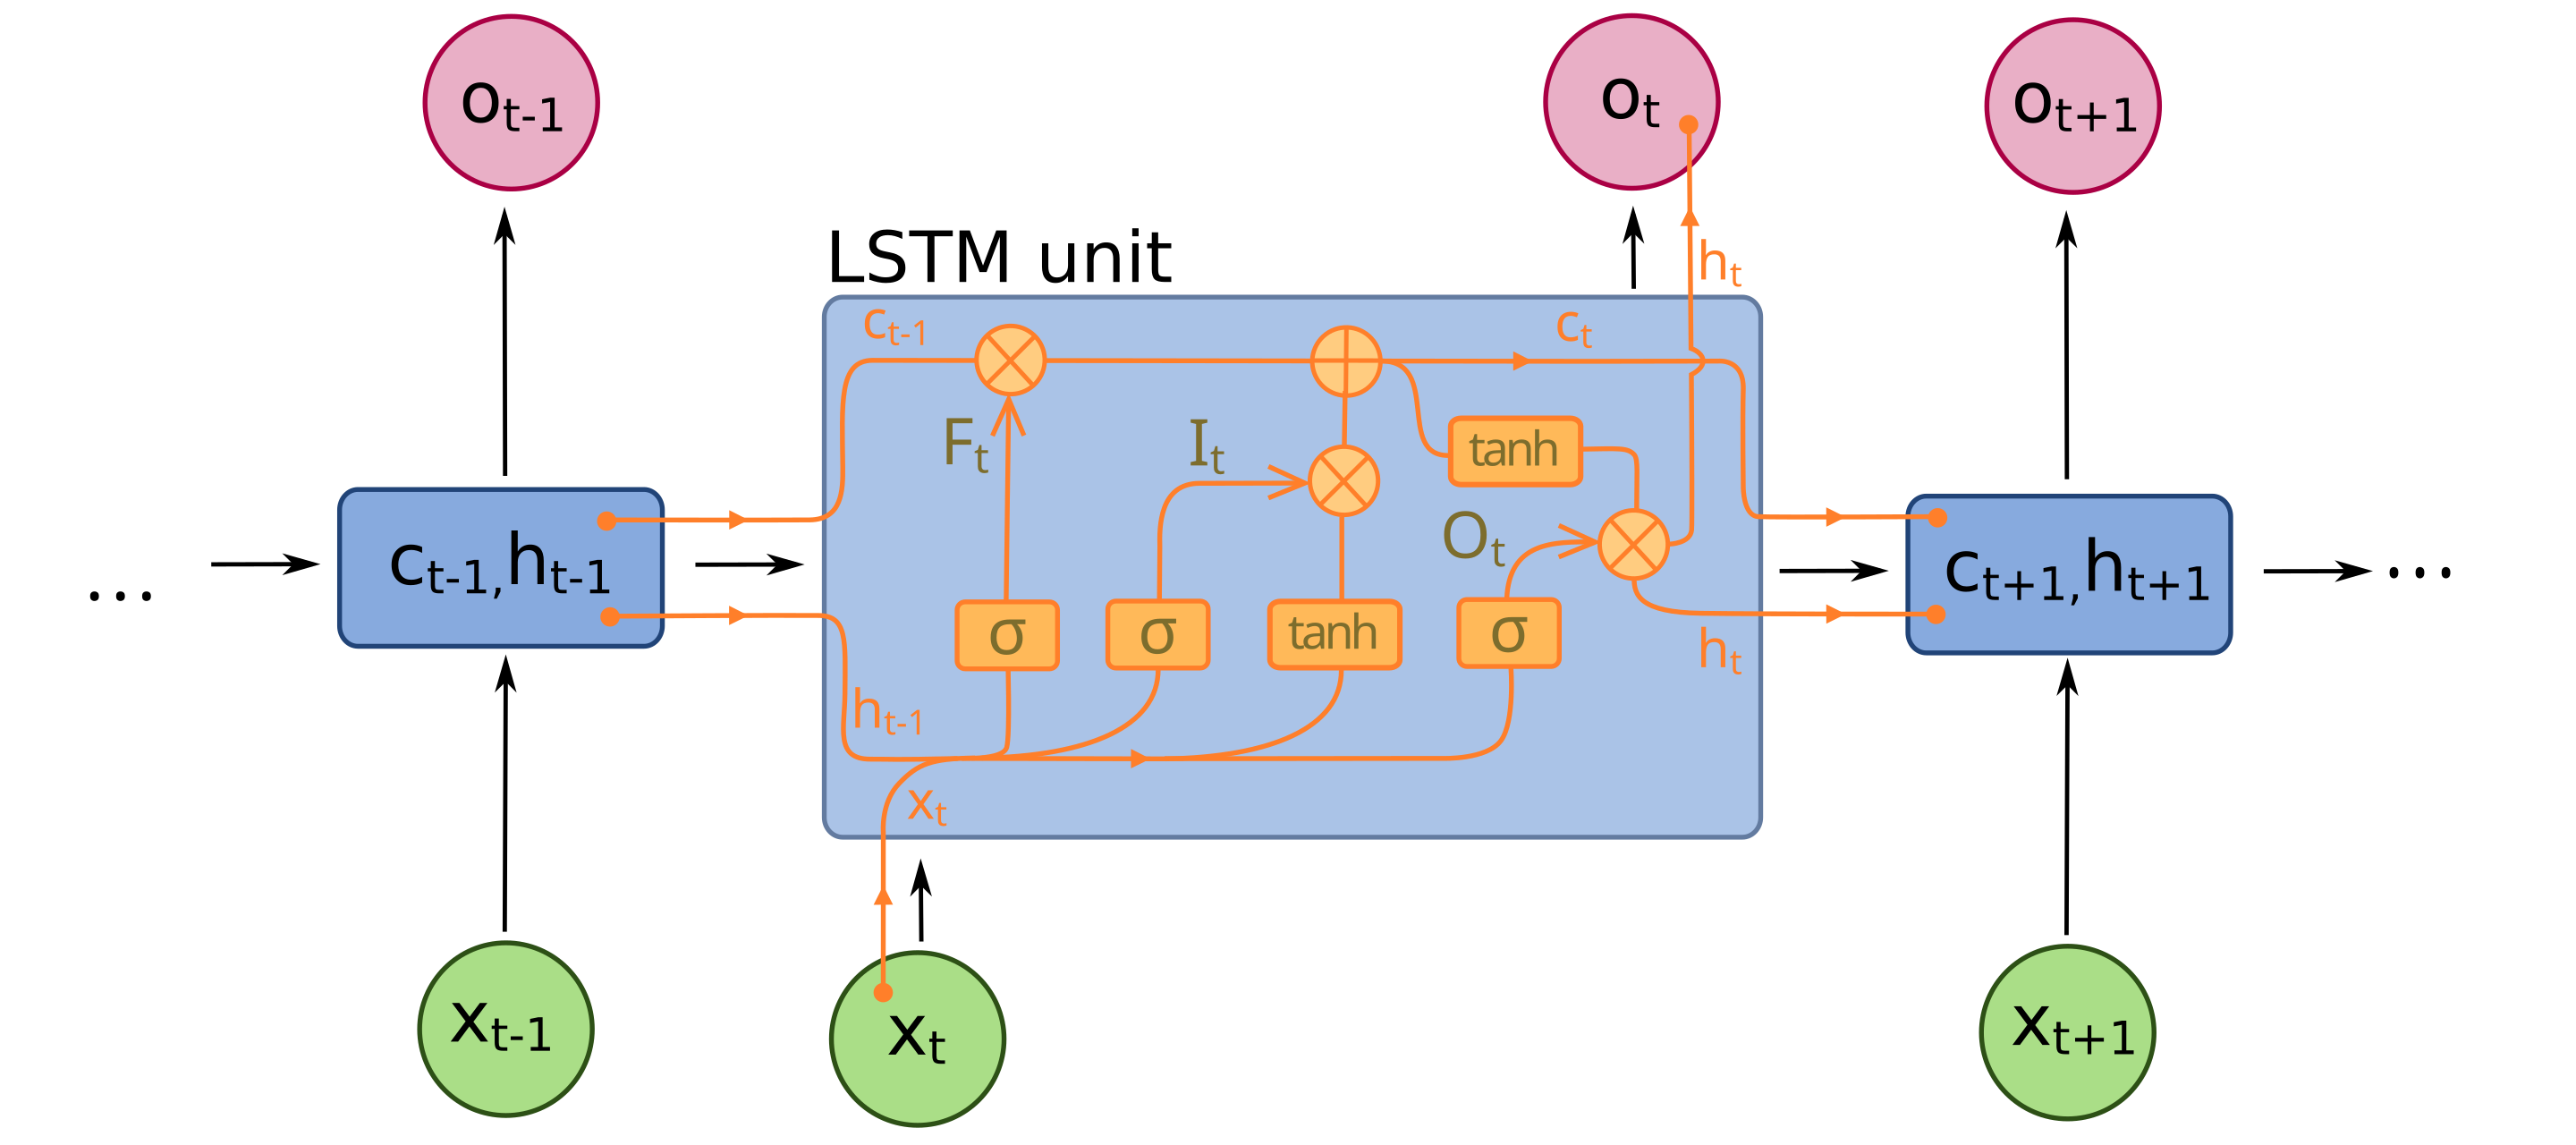
\includegraphics[width=.8\linewidth]{figs/LSTM.png}
        \caption{\tiny Figure by fdeloche\\ \url{https://commons.wikimedia.org/w/index.php?curid=60149410}}
    \end{figure}
    }
    \only<3>{
    \begin{figure}
        \centering
        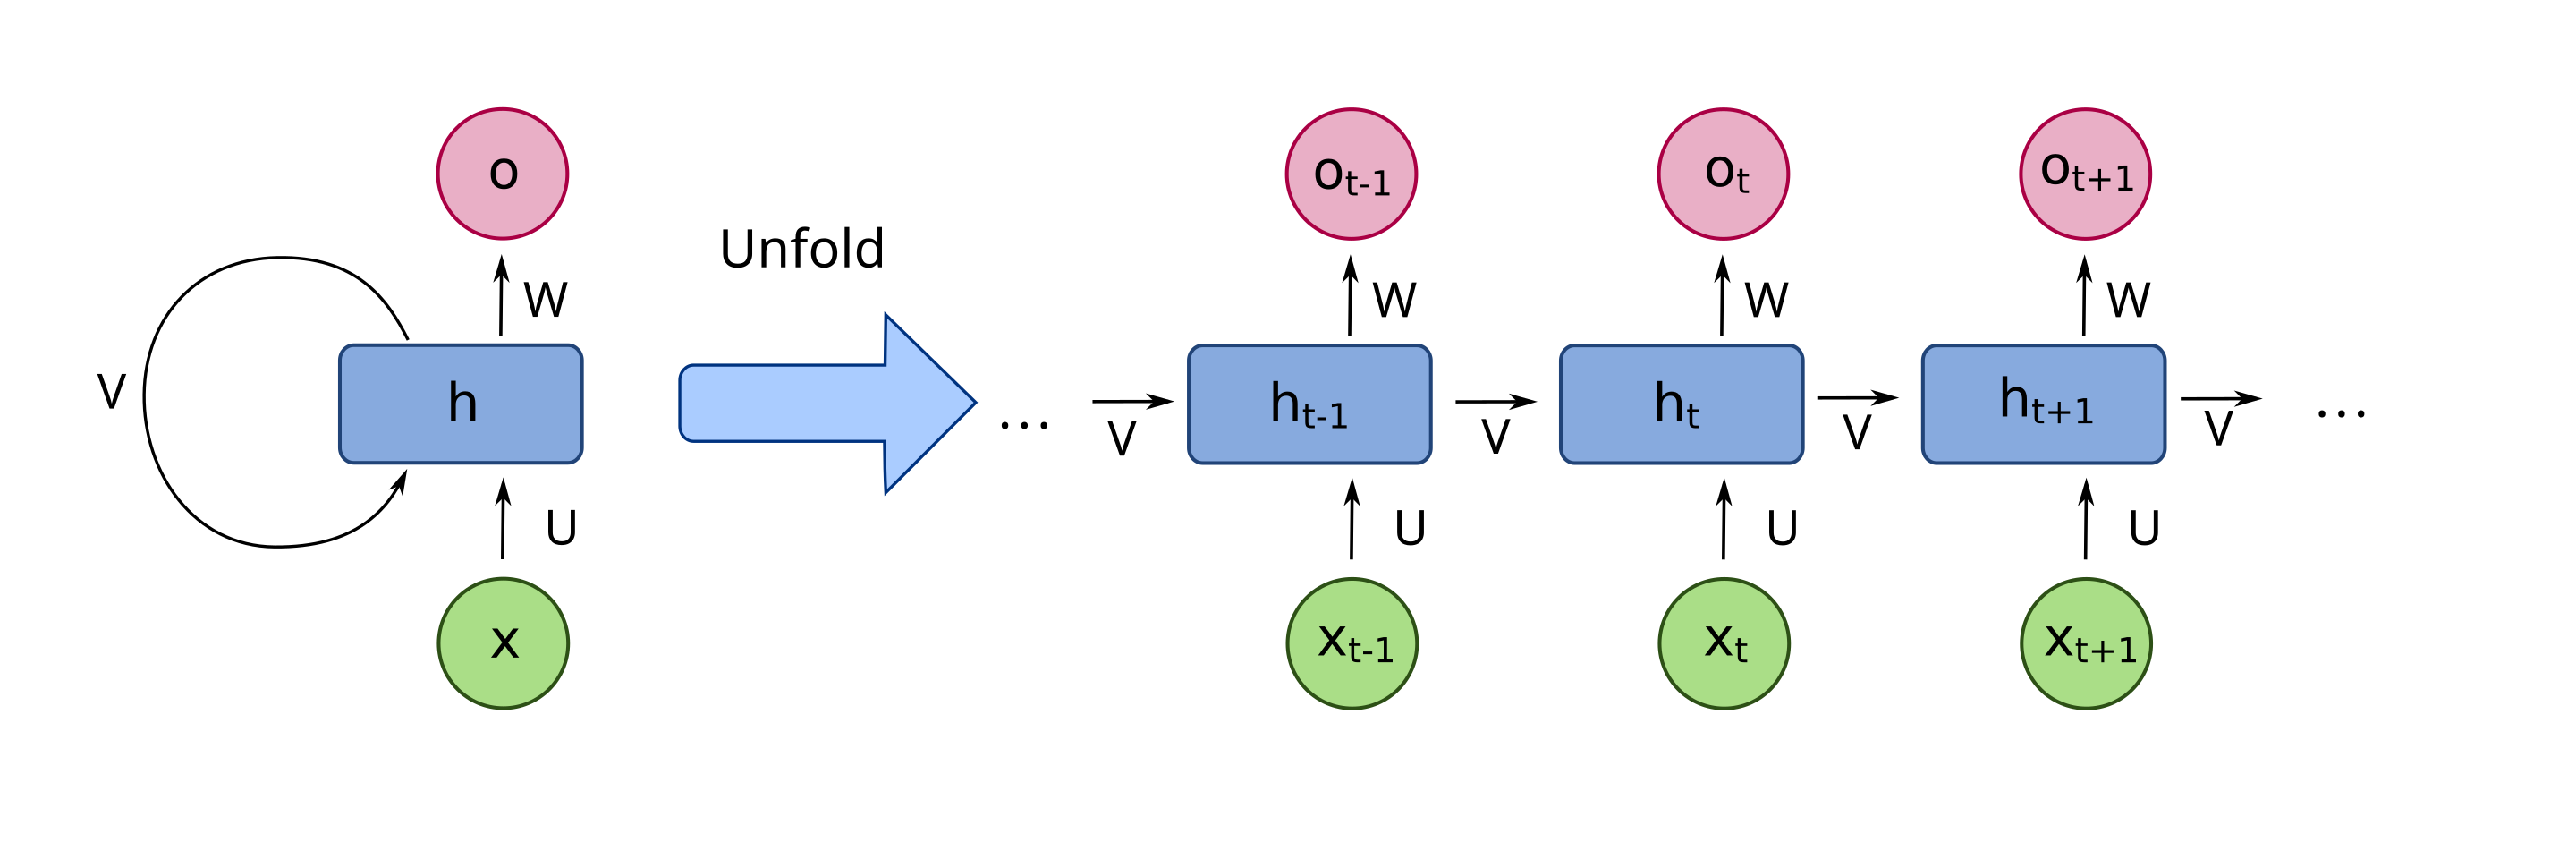
\includegraphics[width=.8\linewidth]{./figs/RNN.png}
        \caption{\tiny Figure by fdeloche\\ \url{https://commons.wikimedia.org/w/index.php?curid=60109157}}
    \end{figure}
    }
\end{columns}
\end{frame}

% Milieu des années 2010 : Évolution vers les Transformateurs et l’Attention
% 8. Transformers - 2017
% Architecture : Transformer (Vaswani et al.)
% Jeu de données paradigmatique : WMT (traduction automatique de l'anglais vers l'allemand), OpenAI GPT sur les jeux de données de génération de texte.
% Optimisation : Adam, un algorithme de descente adaptative, et warmup du taux d’apprentissage, avec une attention particulière sur l'initialisation des poids. Les transformers éliminent complètement la récurrence (comme dans LSTM) en utilisant des mécanismes d'attention auto-régressive.
% Transformers ont révolutionné les tâches de traitement du langage naturel (NLP) en permettant un traitement parallèle des séquences, et ont mené à des modèles comme BERT et GPT.
% 9. GPT (Generative Pretrained Transformers) - 2018-2020
% Architecture : GPT-2, GPT-3 (Radford et al.)
% Jeu de données paradigmatique : WebText, Common Crawl
% Optimisation : Adam, avec des adaptations comme LAMB (Layer-wise Adaptive Moments) pour entraîner des modèles extrêmement larges comme GPT-3 sur des superordinateurs. Le scaling des modèles a rendu nécessaire l’optimisation avancée et la gestion de mémoire.GPT-3 a démontré la puissance des grands modèles linguistiques, capables de générer du texte presque humain, d'accomplir des tâches multiples via un seul modèle entraîné sur des milliards de paramètres.
\begin{frame}[t]{2020's : Transformers ...}
\begin{columns}[t]
    \column{.4\linewidth}
    \vspace{1cm}
    \begin{itemize}
        \item Attention is all you need \cite{vaswani2017attention}
    \end{itemize}
    \column{.6\linewidth}
    \begin{figure}
        \centering
        \vspace{-1.5cm}
        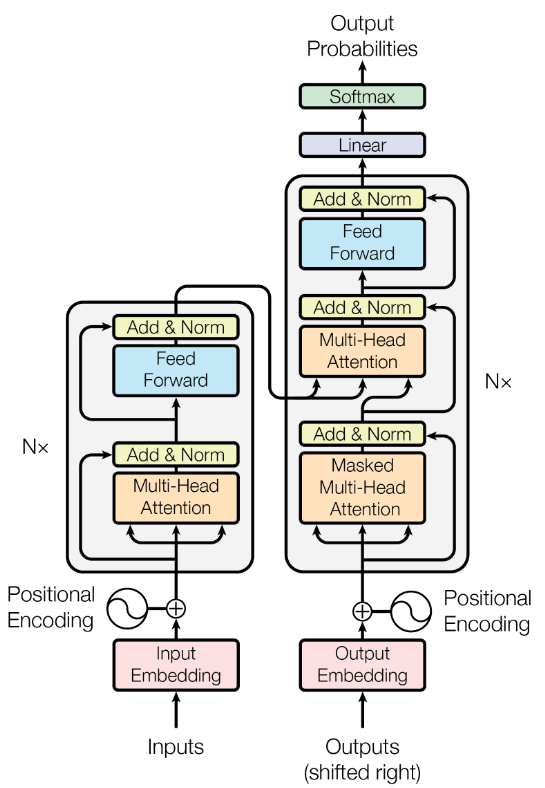
\includegraphics[width=.6\linewidth]{figs/transformer.png}
        \caption{\tiny A transformer block. Figure from \cite{vaswani2017attention}}
    \end{figure}
\end{columns}
\end{frame} 

\begin{frame}{Sidestep : Transformers}
        \centering
    \begin{figure}
        \centering
        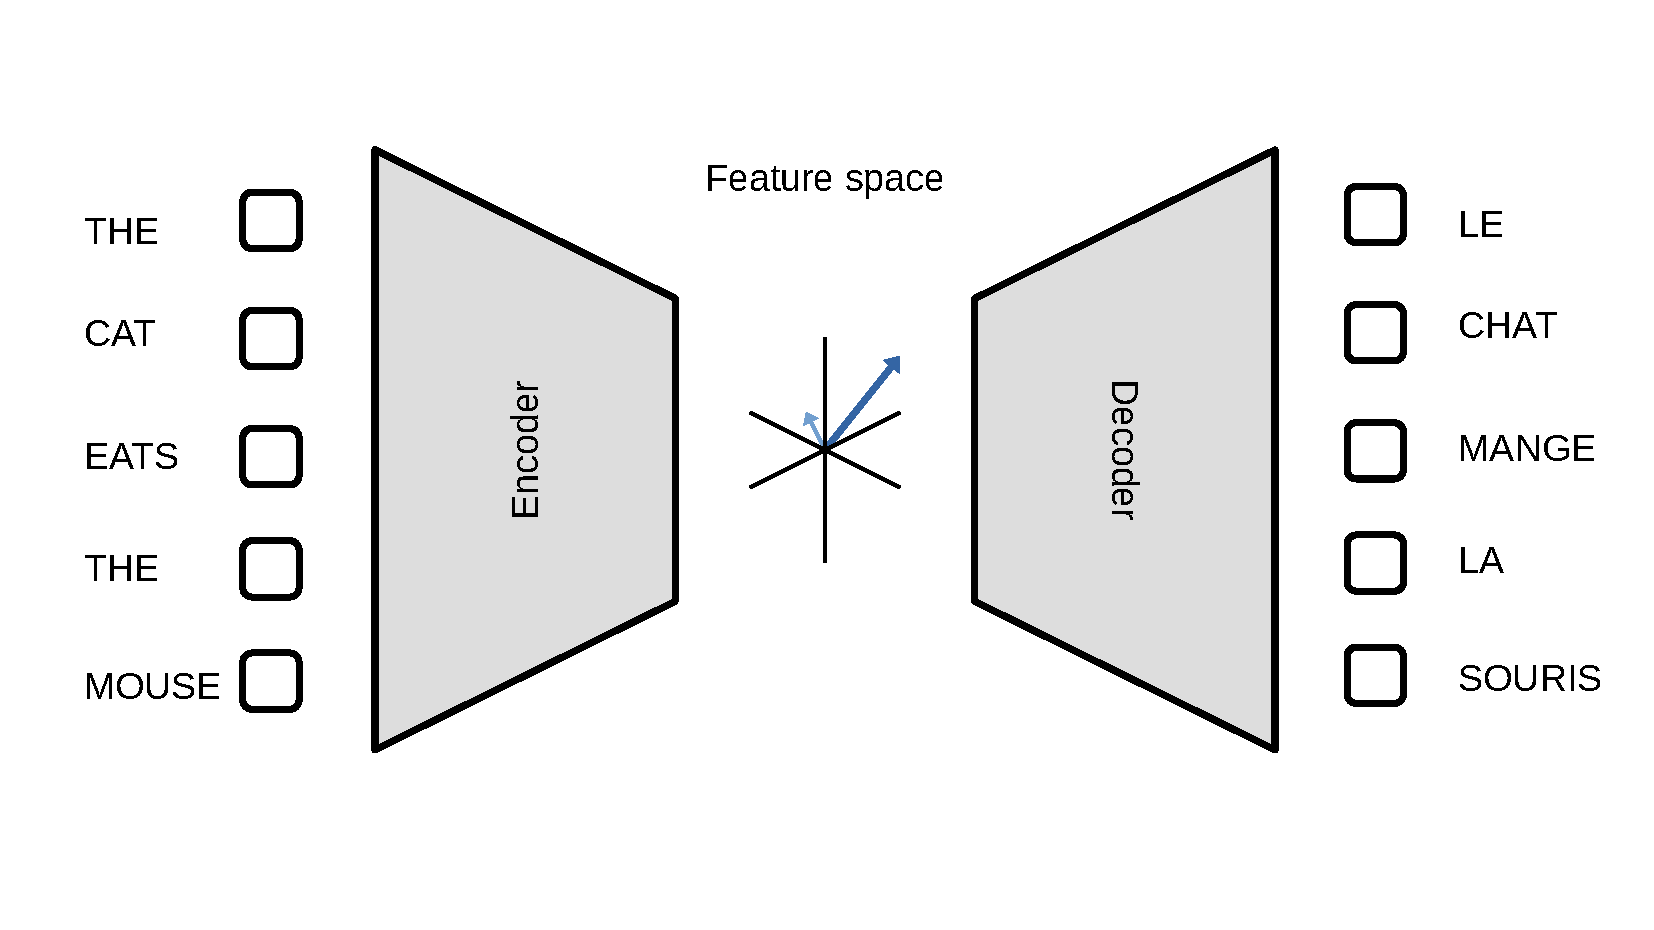
\includegraphics[width=.7\linewidth]{./figs/encoder_decoder.pdf}
    \end{figure}
\end{frame}


\begin{frame}{Sidestep : Transformers}
        \centering
    \begin{figure}
        \centering
        \includegraphics<1>[width=.5\linewidth]{figs/attention1.png}%
        \includegraphics<2>[width=.5\linewidth]{figs/attention2.png}%
        \includegraphics<3>[width=.5\linewidth]{figs/attention3.png}%
    \end{figure}
    \only<1>{\textcolor{darkblue}{The knight} \textcolor{black}{saves} \textcolor{blue}{the queen}}%
    \only<2>{\textcolor{blue}{Queen} \textcolor{black}{takes} \textcolor{darkblue}{knight} \textcolor{red}{, checkmate !}}%
    \only<3>{\textcolor{black}{He was} \textcolor{darkblue}{knighted} \textcolor{black}{by} \textcolor{blue}{Queen} \textcolor{red}{Elizabeth II}}%
\end{frame}

\begin{frame}{Sidestep : Transformers}
        \centering
    \begin{figure}
        \centering
        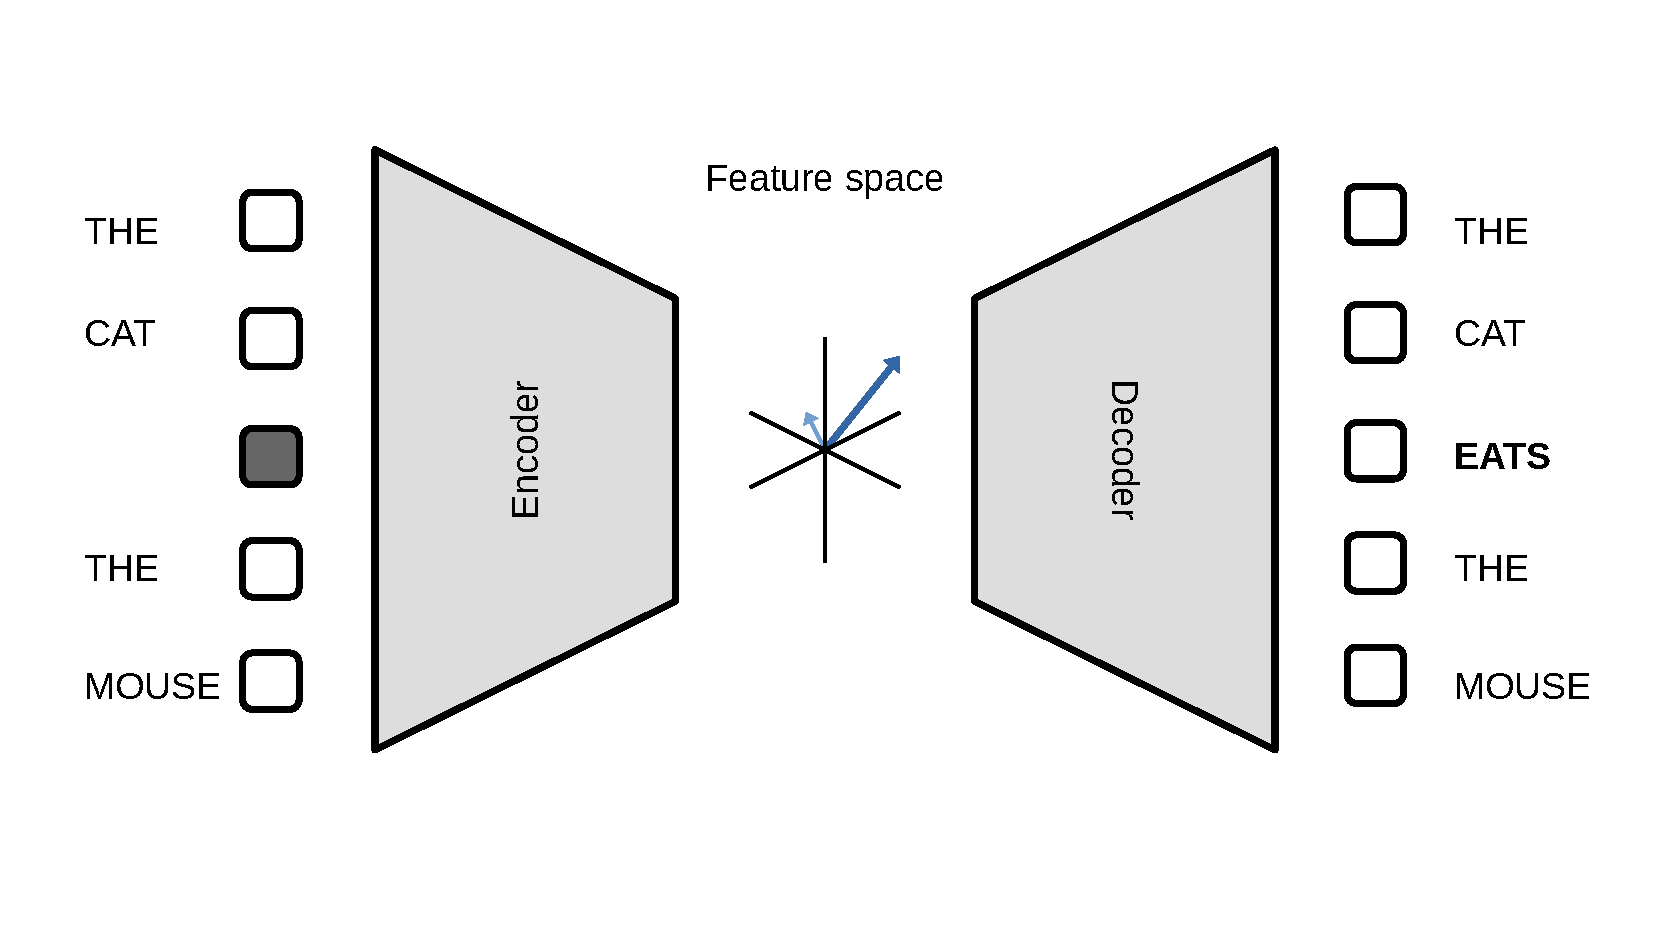
\includegraphics[width=.7\linewidth]{./figs/mae.pdf}
    \end{figure}
\end{frame}

% 2020 et au-delà : Évolution des Grands Modèles et Vision Transformer
% 10. Vision Transformers (ViT) - 2020
% Architecture : ViT (Dosovitskiy et al.)
% Jeu de données paradigmatique : ImageNet, JFT-300M
% Optimisation : AdamW (Adam avec pondération de décroissance), et des variantes comme Lookahead pour stabiliser l'apprentissage des grands réseaux basés sur l'attention.
% ViT a montré que les transformers peuvent également surpasser les CNN classiques sur les tâches de vision par ordinateur, remplaçant progressivement les architectures convolutives dans certaines applications.
\begin{frame}[t]{2020's : Transformers ... and Self Supervised Learning}
\begin{columns}[t]
    \column{.4\linewidth}
    \vspace{1cm}
    \begin{itemize}
        \item Attention is all you need\\ \cite{vaswani2017attention}
        \item LLMs (GPT, BERT...)\\ \cite{devlin2019bert}
    \end{itemize}
    \column{.6\linewidth}
    \begin{figure}
        \centering
        
\includegraphics[width=.7\linewidth]{figs/llms.png}
        \caption{\tiny caption}
    \end{figure}
\end{columns}
\end{frame} 

\begin{frame}[t]{2020's : Transformers ... and Self Supervised Learning}
\begin{columns}[t]
    \column{.4\linewidth}
    \vspace{1cm}
    \begin{itemize}
        \item<1-> Vision Transformer\\ \cite{dosovitskiy2020image}
        \item<2-> Masked Auto Encoder\\ \cite{he2022masked}
        \item<3-> DINO\\ \cite{caron2021emerging}
    \end{itemize}
    \column{.6\linewidth}
    \only<1>{
    \begin{figure}
        \centering
        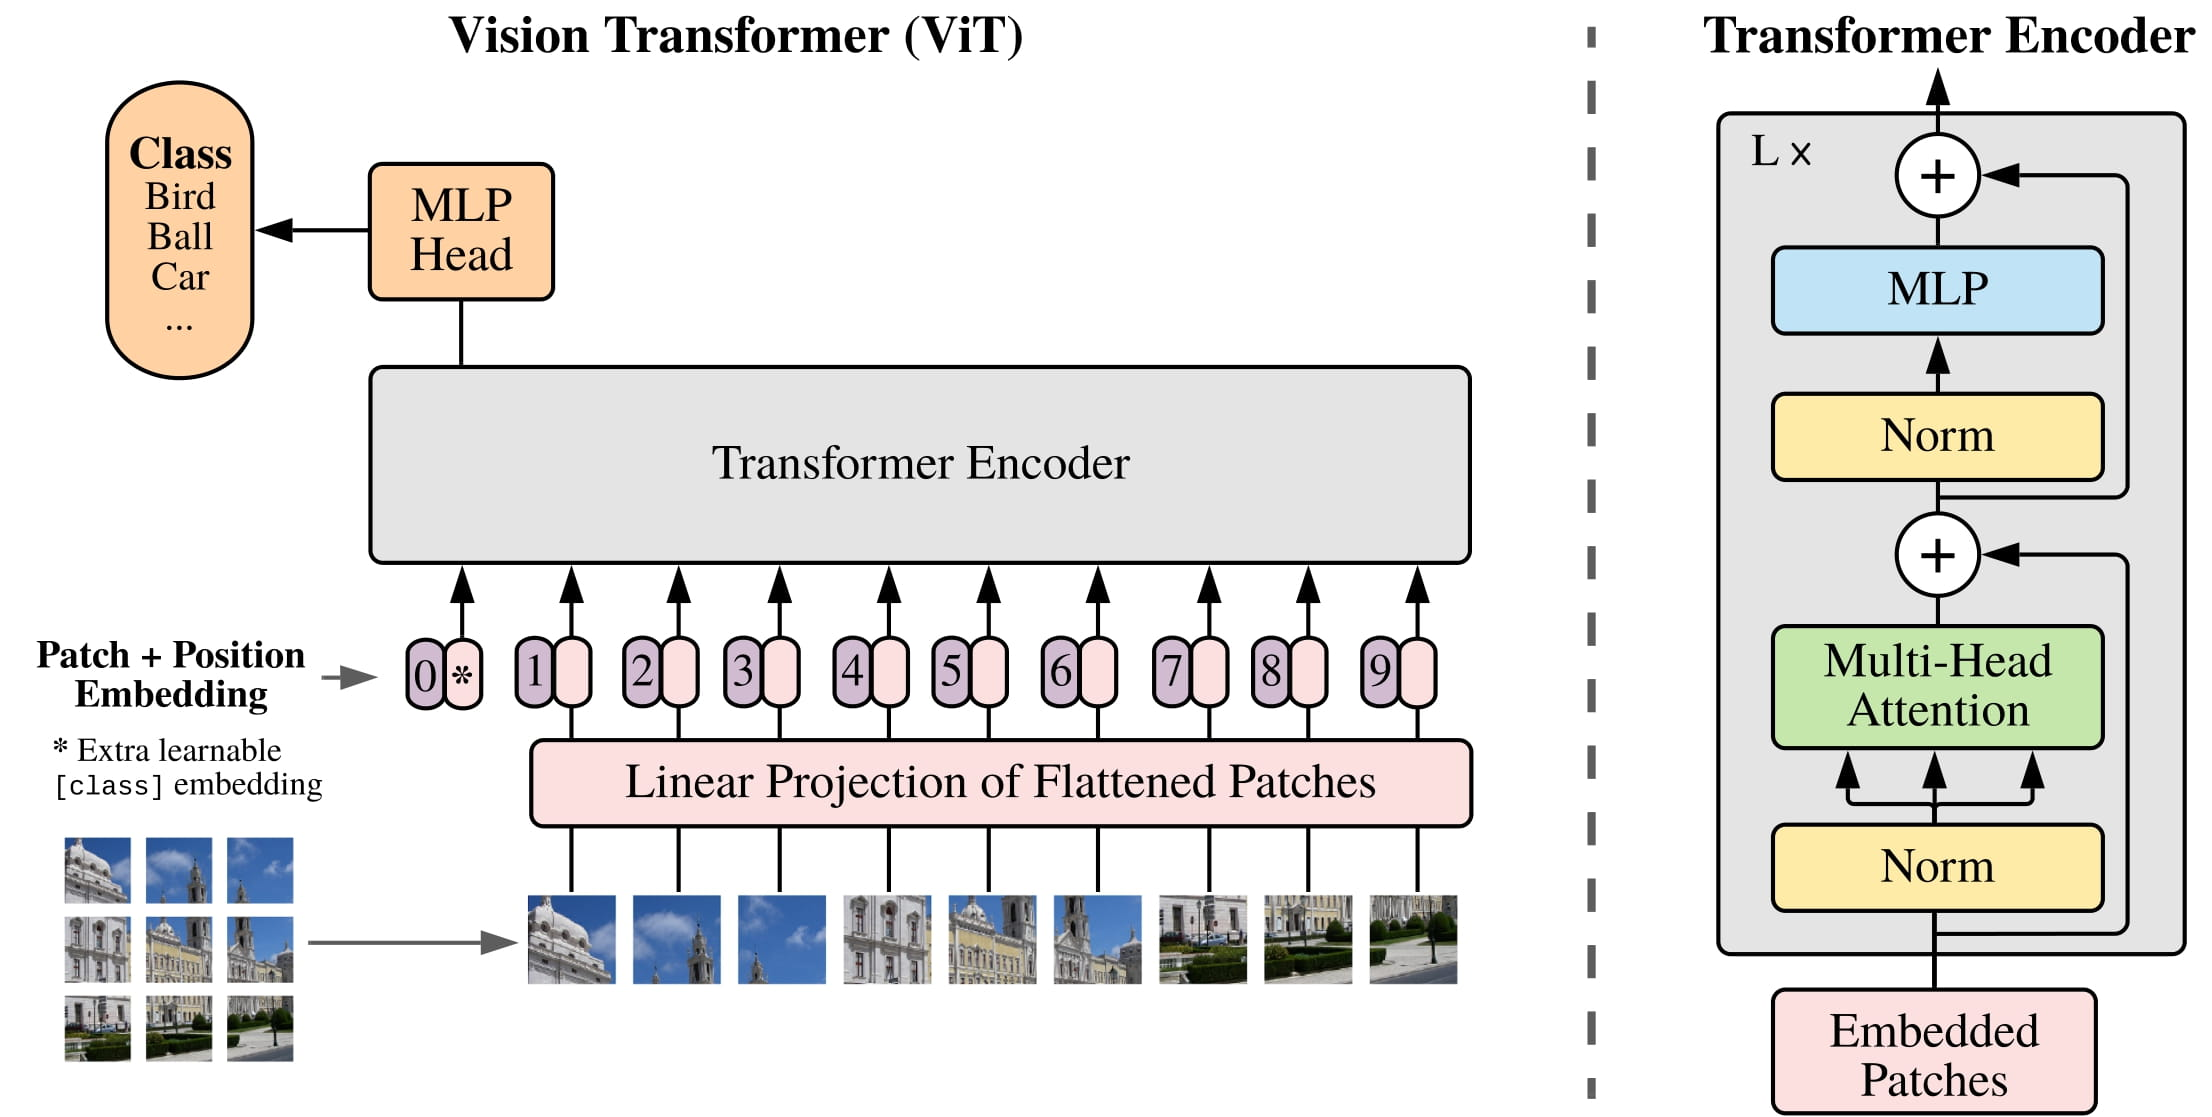
\includegraphics[width=\linewidth]{figs/vit.jpg}
        \caption{\tiny Figure from \cite{dosovitskiy2020image} }
    \end{figure}
    }
    \only<2>{
    \begin{figure}
        \centering
        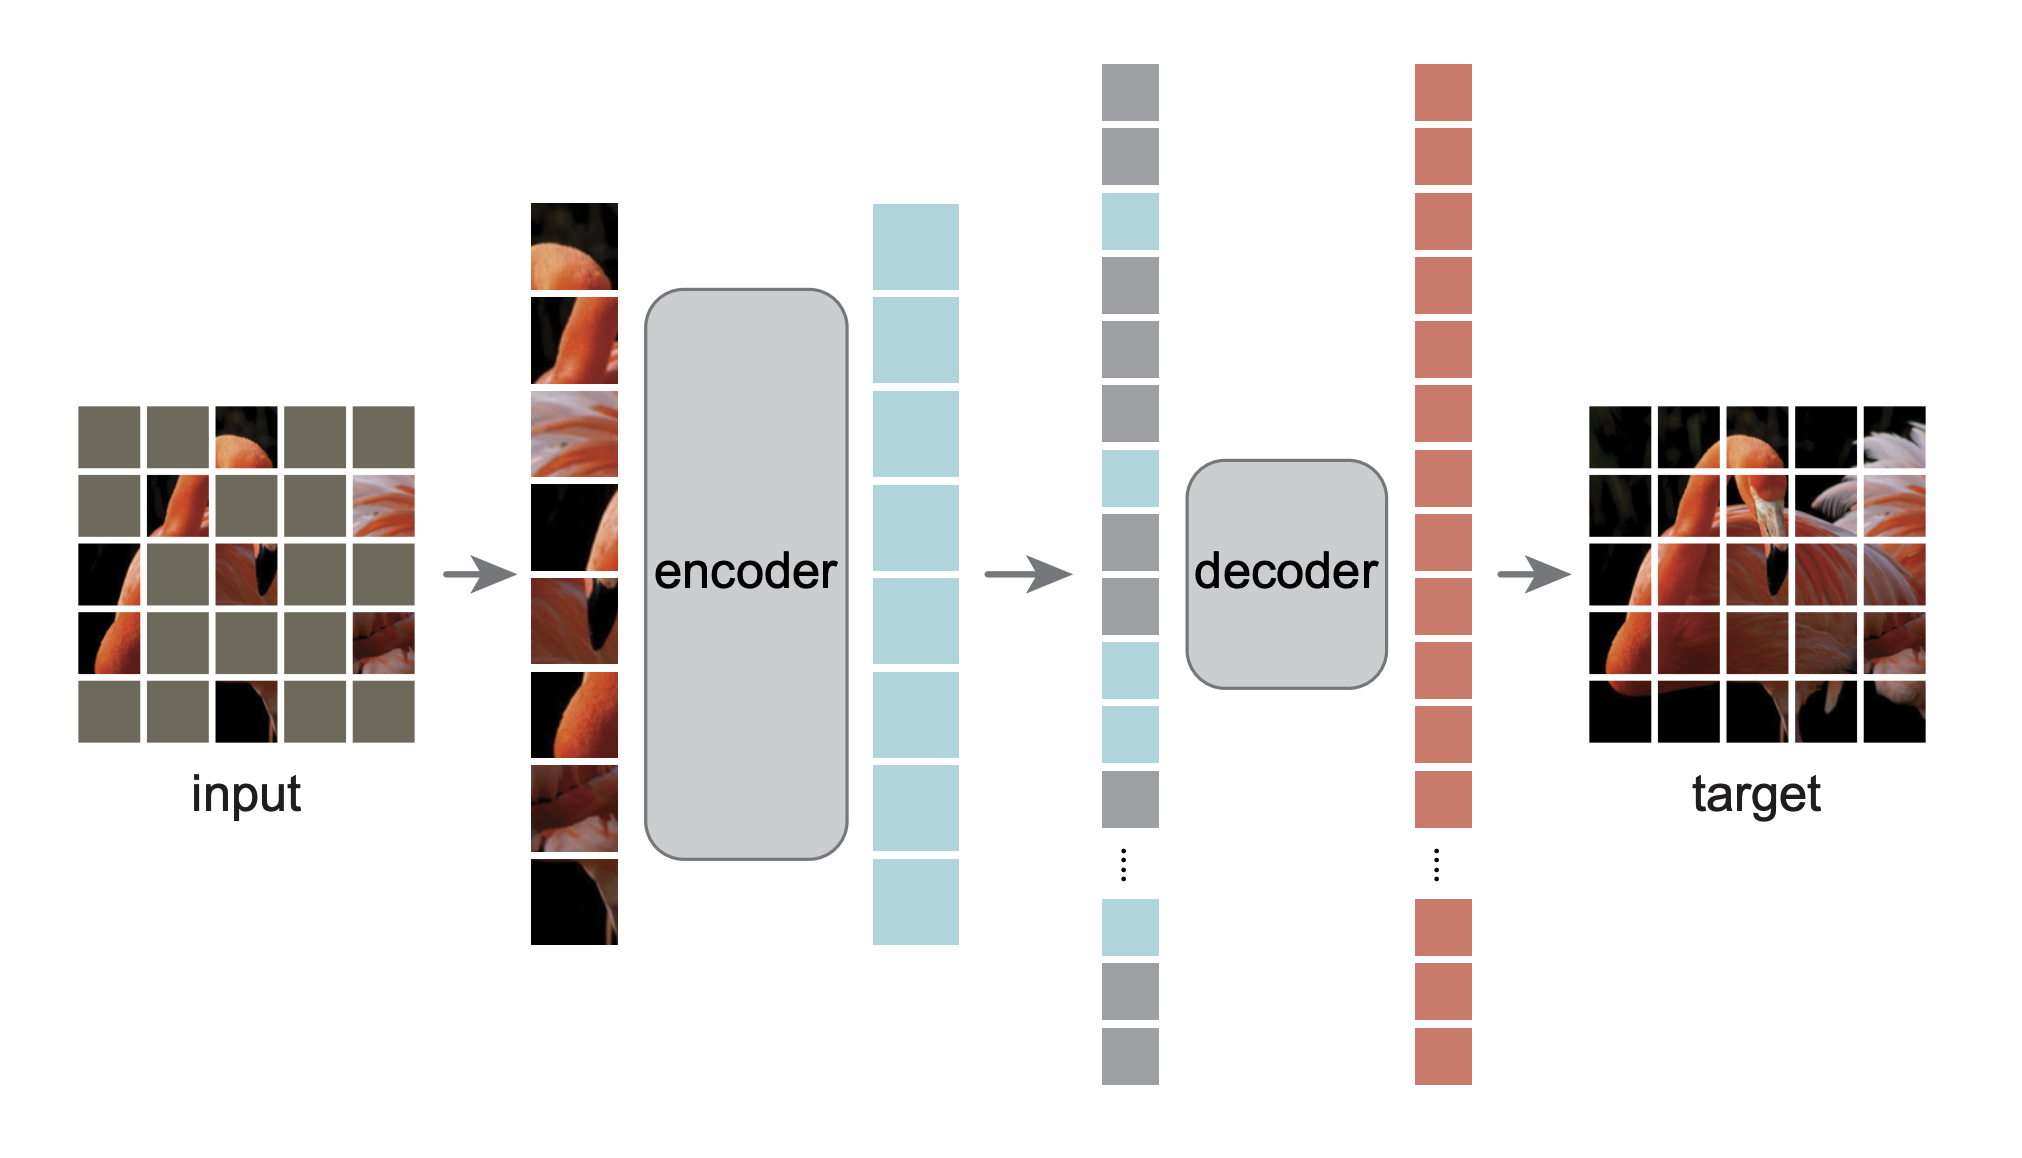
\includegraphics[width=.8\linewidth]{figs/mae.png}
        \caption{\tiny Figure from \cite{he2022masked}}
    \end{figure}
    }
    \only<3>{
    \begin{figure}
        \centering
        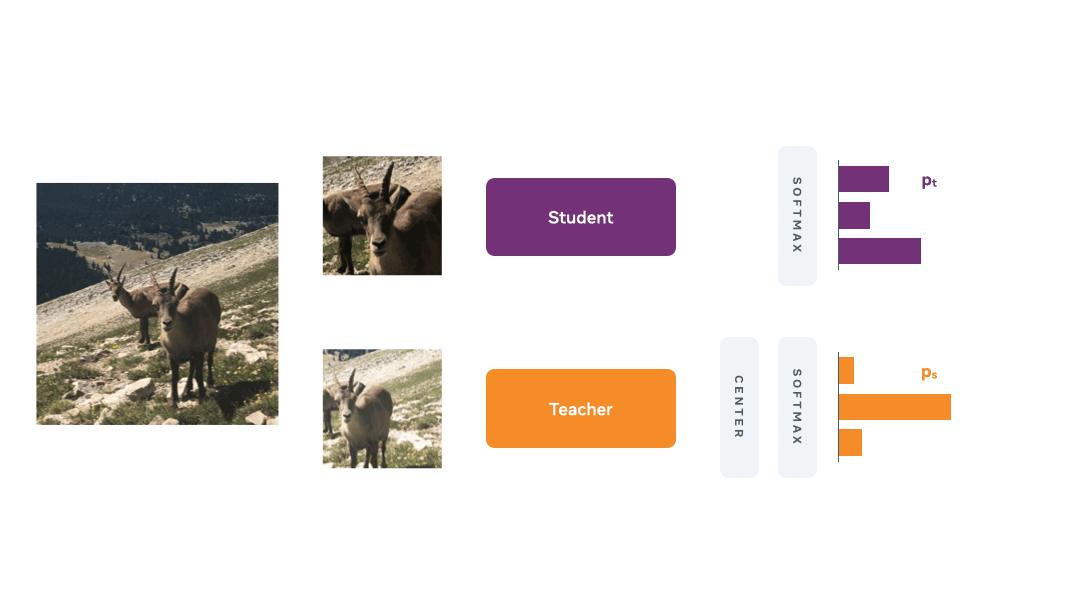
\includegraphics[width=.8\linewidth]{./figs/dino3.png}
        \caption{\tiny Figure from \cite{caron2021emerging}}
    \end{figure}
    }
\end{columns}
\end{frame} 

\begin{frame}{A lot left out !}
\begin{center}
    \begin{tikzpicture}[remember picture, overlay]
        % Define coordinates for the words
        \coordinate (word1) at (-2.5, 3);
        \coordinate (word2) at (-4, 2);
        \coordinate (word3) at (3, 4);
        \coordinate (word4) at (-3, -2);
        \coordinate (word5) at (2, -2);
        \coordinate (word6) at (-2, 1);
        \coordinate (word7) at (1.5, -1);
        \coordinate (word8) at (3, -3);

        % Overlay words using \node and \only
        \only<1->{\node[font=\bfseries] at (word1) {Finetuning};}
        \only<2->{\node[font=\bfseries] at (word2) {Games};}
        \only<3->{\node[font=\bfseries] at (word3) {Reinforcement learning};}
        \only<4->{\node[font=\bfseries] at (word4) {Time series};}
        \only<5->{\node[font=\bfseries] at (word5) {Speech recognition};}
        \only<6->{\node[font=\bfseries] at (word6) {Image generation};}
        \only<7->{\node[font=\bfseries] at (word7) {Diffusion models};}
        \only<8->{\node[font=\huge\bfseries] at (word8) {...};}
    \end{tikzpicture}
\end{center}
\end{frame}

\begin{frame}{Usefull ressources}
\begin{columns}[t]
    \column{.5\linewidth}
    \textbf{State of the art}
    \begin{itemize}
        \item \href{https://huggingface.co/}{Huggingface}
        \item \href{https://paperswithcode.com/sota}{PapersWithCode}
    \end{itemize}
    \textbf{Getting started}
    \begin{itemize}
        \item \href{https://docs.pytorch.org/tutorials/}{Pytorch}
        \item \href{https://keras.io/getting_started/}{Keras}
    \end{itemize}
    \column{.5\linewidth}
    \textbf{Understanding papers}
    \begin{itemize}
        \item \href{https://www.youtube.com/@YannicKilcher}{Yannic Kilcher}
        \item \href{https://www.youtube.com/@AICoffeeBreak}{AI coffe break}
    \end{itemize}
    \textbf{Understanding visually}
    \begin{itemize}
        \item \href{https://www.youtube.com/@3blue1brown}{3blue1brown}
        \item \href{https://www.youtube.com/@Deepia-ls2fo}{deepia}
    \end{itemize}
\end{columns}

\end{frame}

\begin{frame}[plain]
    \Huge{\textbf{Thanks for you attention !}}
    
    \vfill
    
    \LARGE{\textbf{Let's practice !}}
\end{frame}

\appendix
% \printbibliography
% [heading=none]
\begin{frame}[allowframebreaks]{References}
\setbeamertemplate{bibliography item}{}
    {\footnotesize \printbibliography[heading=none]}
\end{frame}


\end{document}
